\subsection{Results for $C_{DS}=0.0$}
The following results are for a run with the following input conditions:
\begin{longtable}[c]{A{3.0cm}  A{3.0cm}}
    \caption{Input list for $C_{DS}=0$ test}    \\  \hline
        \textbf{Parameter}      &       \textbf{Value}      \\  \hline
    \endfirsthead
    \caption{Input list for $C_{DS}=0$ test~(continued)}    \\  \hline
        \textbf{Parameter}      &       \textbf{Value}      \\  \hline
    \endhead
        $N$                 &   64      \\
        $t_{final}$         &   100.0   \\
        $C_{DS}$            &   0.0     \\
        $C_{BS}$            &   1.0     \\
\end{longtable}

%\newpage

\begin{figure}[H]
    \begin{subfigure}[H]{0.45\textwidth}
        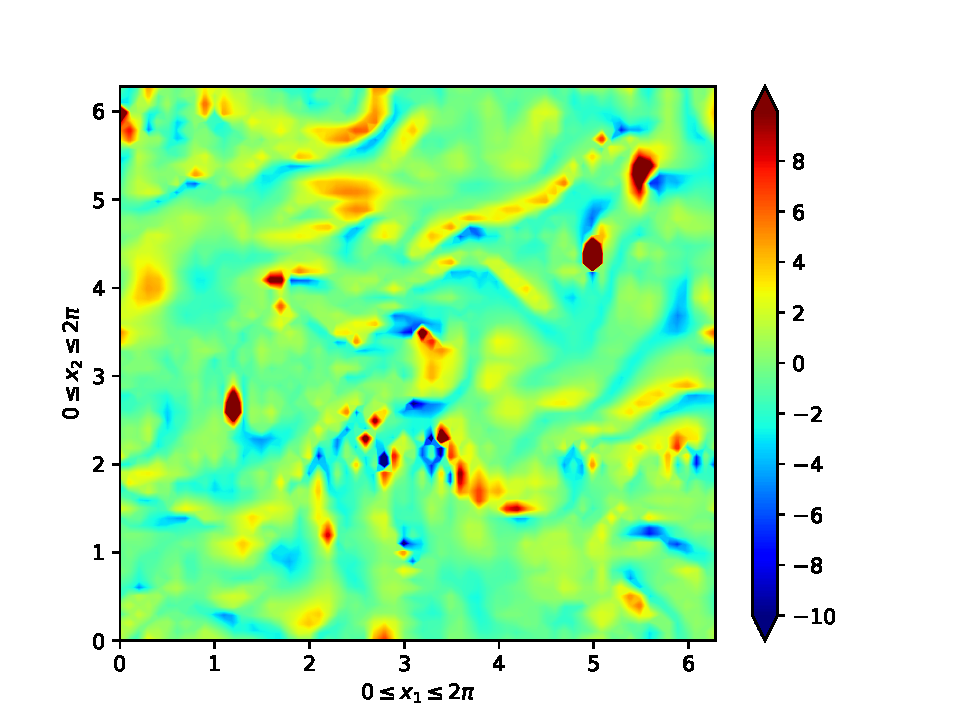
\includegraphics[height=1.75in]{media/run-cds-00/ke-RHS-CDS-00}
        \caption{$\frac{1}{k} \frac{Dk}{Dt}$}
    \end{subfigure}
    ~
    \begin{subfigure}[H]{0.45\textwidth}
        \includegraphics[height=1.75in]{media/run-cds-00/enstrophy-RHS-CDS-00}
        \caption{$\frac{1}{\Omega} \frac{D \Omega}{Dt}$}
    \end{subfigure}
    \newline
    \begin{subfigure}{0.45\textwidth}
        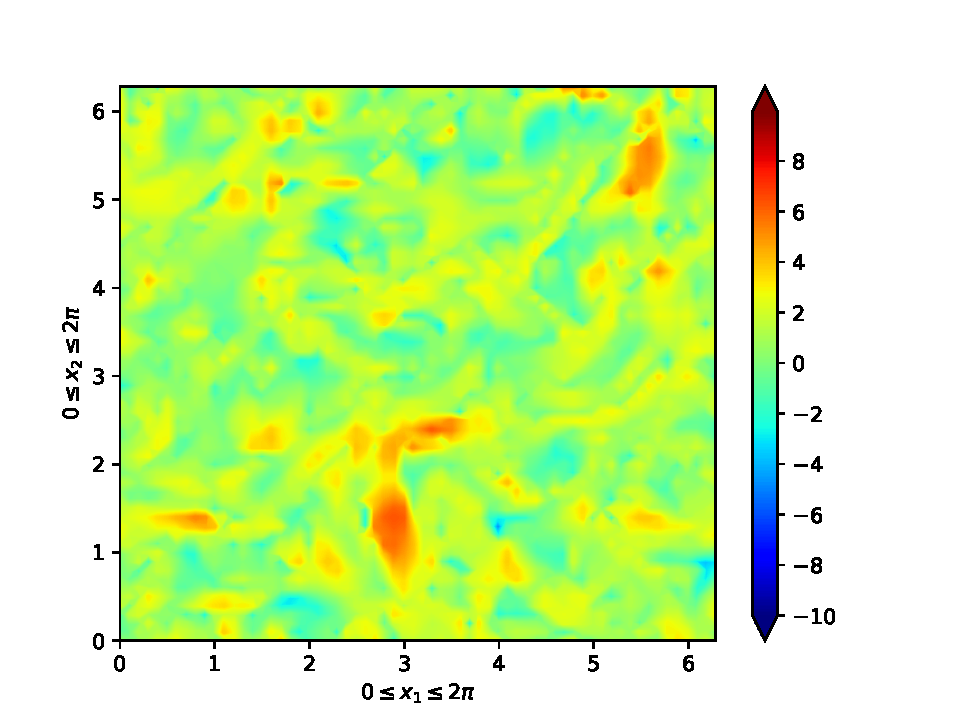
\includegraphics[height=1.75in]{media/run-cds-00/A-enst-CDS-00}
        \caption{$A$}
    \end{subfigure}
    ~
    \begin{subfigure}{0.45\textwidth}
        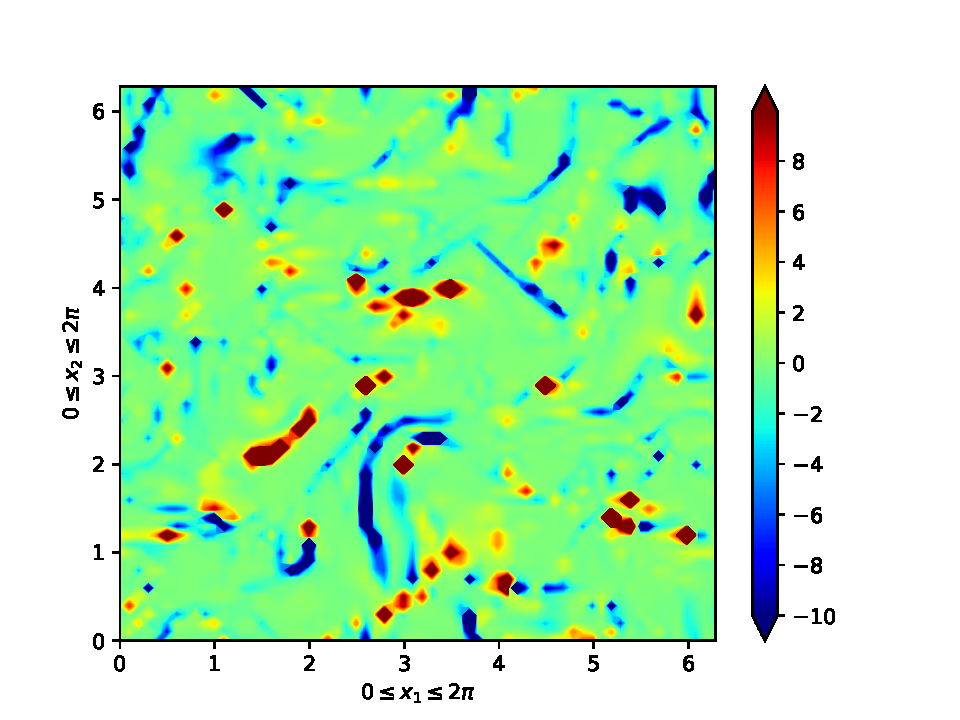
\includegraphics[height=1.75in]{media/run-cds-00/trans-enst-CDS-00}
        \caption{$\Pi$}
    \end{subfigure}
    \newline
    \begin{subfigure}{0.45\textwidth}
        \includegraphics[height=1.75in]{media/run-cds-00/prod-enst-CDS-00}
        \caption{$P$}
    \end{subfigure}
    ~
    \begin{subfigure}{0.45\textwidth}
        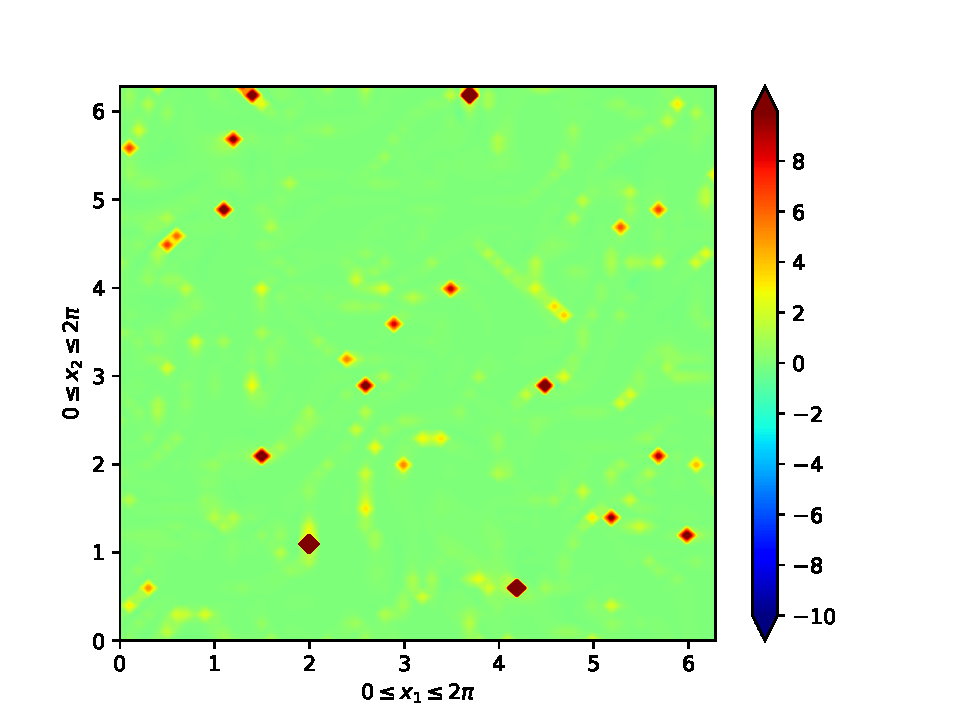
\includegraphics[height=1.75in]{media/run-cds-00/B-enst-CDS-00}
        \caption{$B$}
    \end{subfigure}
    \newline
    \begin{subfigure}{0.45\textwidth}
        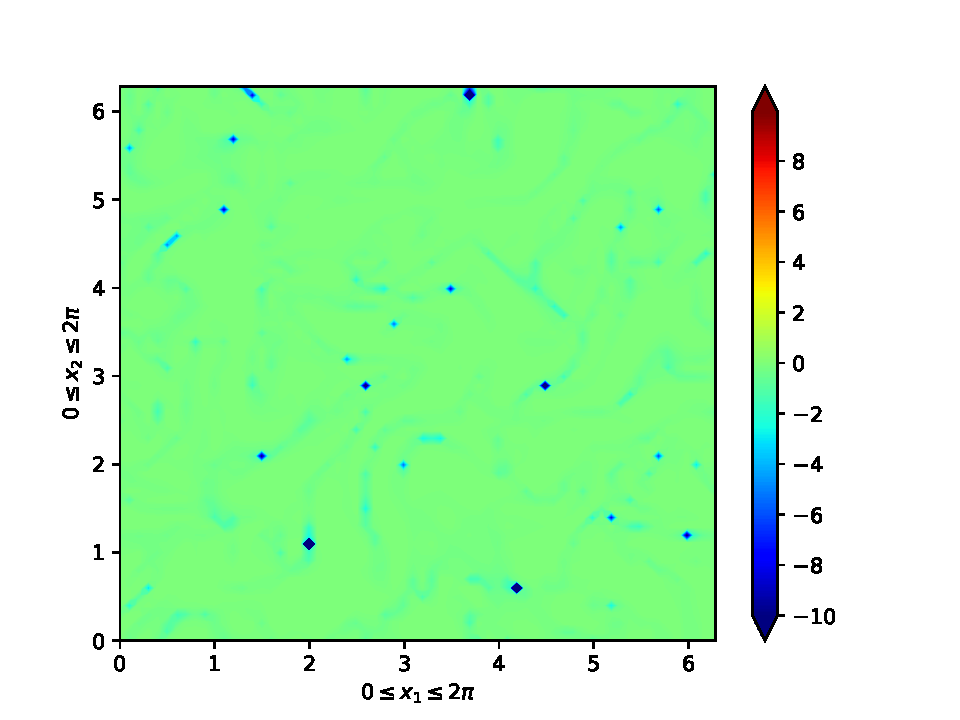
\includegraphics[height=1.75in]{media/run-cds-00/D-enst-CDS-00}
        \caption{$D$}
    \end{subfigure}
\end{figure}
%\newpage

%------------------------------------------------------------------------------%
% C_{DS} = 0.65                                                                %
%------------------------------------------------------------------------------%
\subsection{Results for $C_{DS}=0.65$}
%------------------------------------------------------------------------------%
% 1310                                                                         %
%------------------------------------------------------------------------------%
\subsubsection{$t=29.81$ i.e., $t=t^{\ast} - 10\Delta t$} 
\begin{figure}[H]
    \begin{subfigure}[H]{0.45\textwidth}
        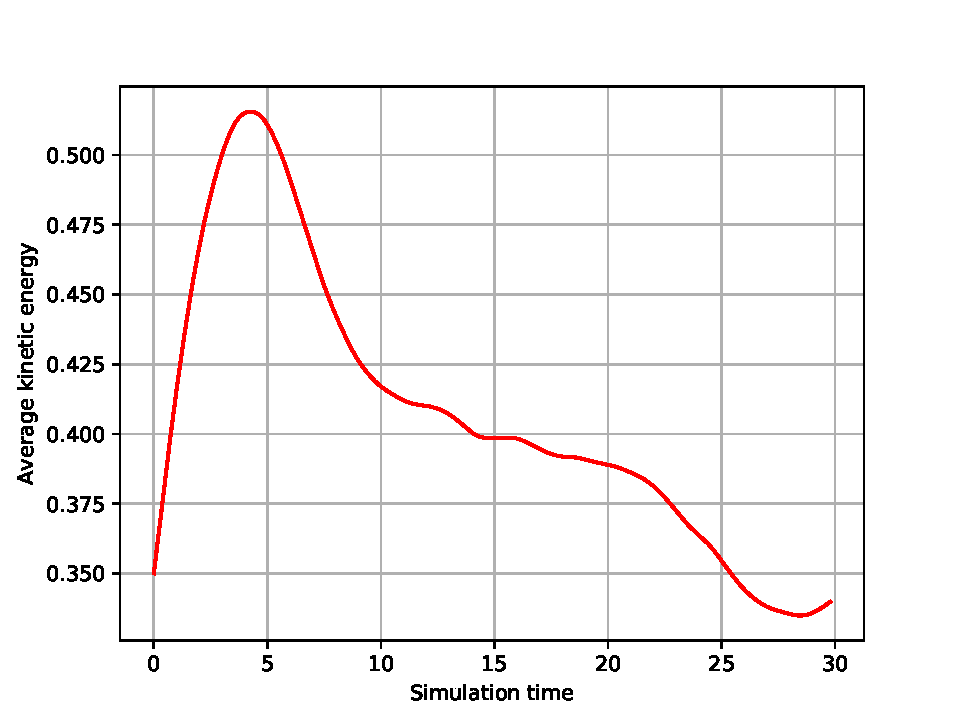
\includegraphics[height=1.75in]{media/run-cds-65/ke-average1310}
        \caption{Average kinetic energy}
    \end{subfigure}
    ~
    \begin{subfigure}[H]{0.45\textwidth}
        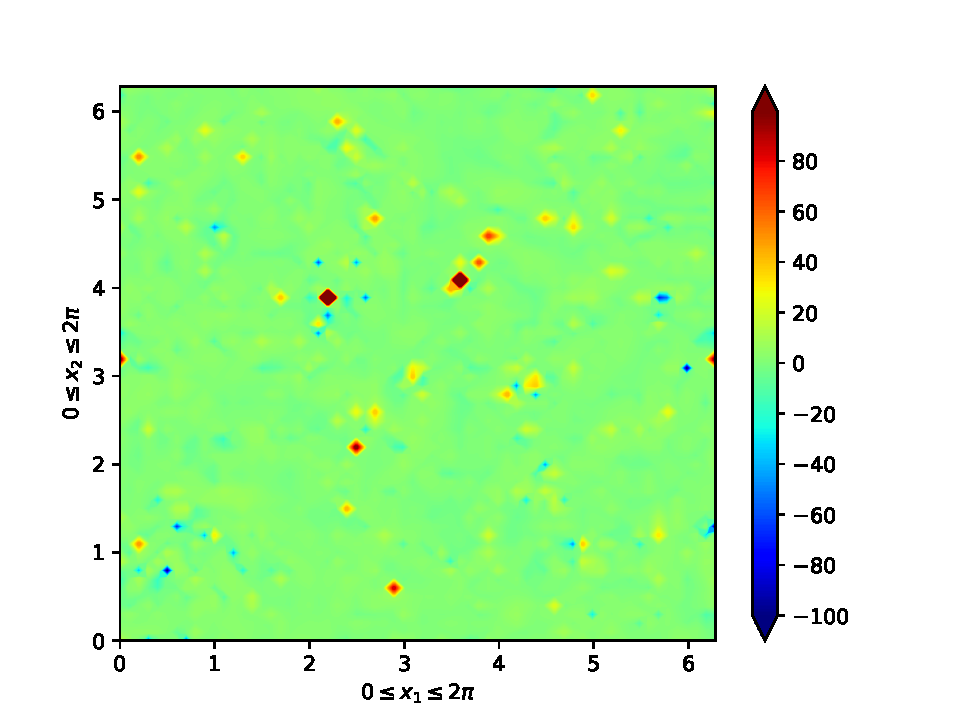
\includegraphics[height=1.75in]{media/run-cds-65/enst-1310}
        \caption{$\frac{1}{\Omega} \frac{D \Omega}{Dt}$}
    \end{subfigure}
    \newline
    \begin{subfigure}{0.45\textwidth}
        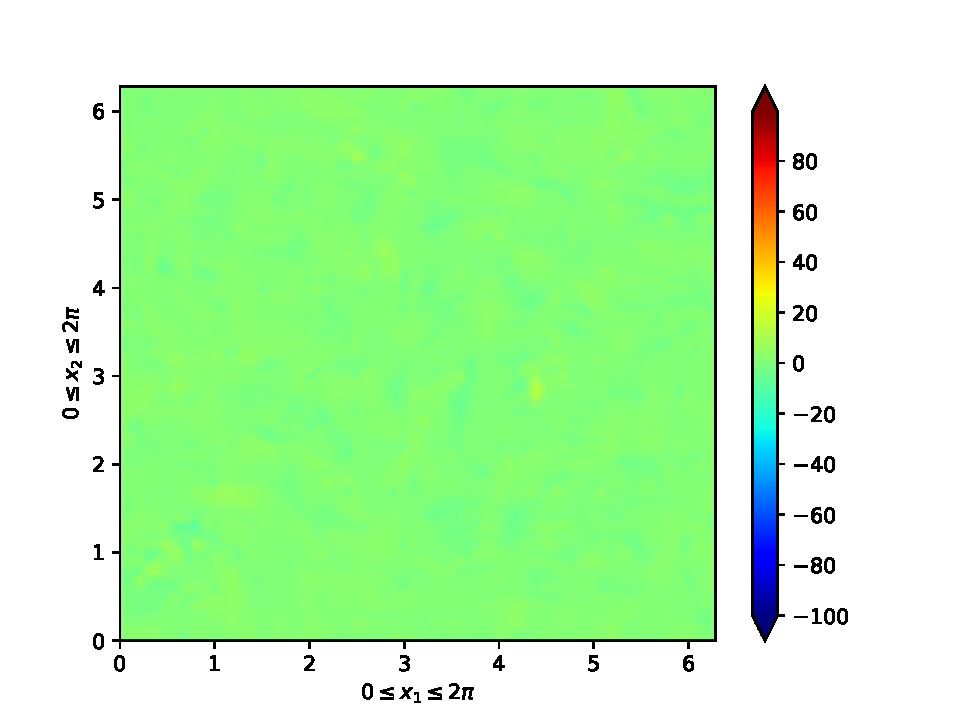
\includegraphics[height=1.75in]{media/run-cds-65/A-enst-1310}
        \caption{$A_{\Omega}$}
    \end{subfigure}
    ~
    \begin{subfigure}{0.45\textwidth}
        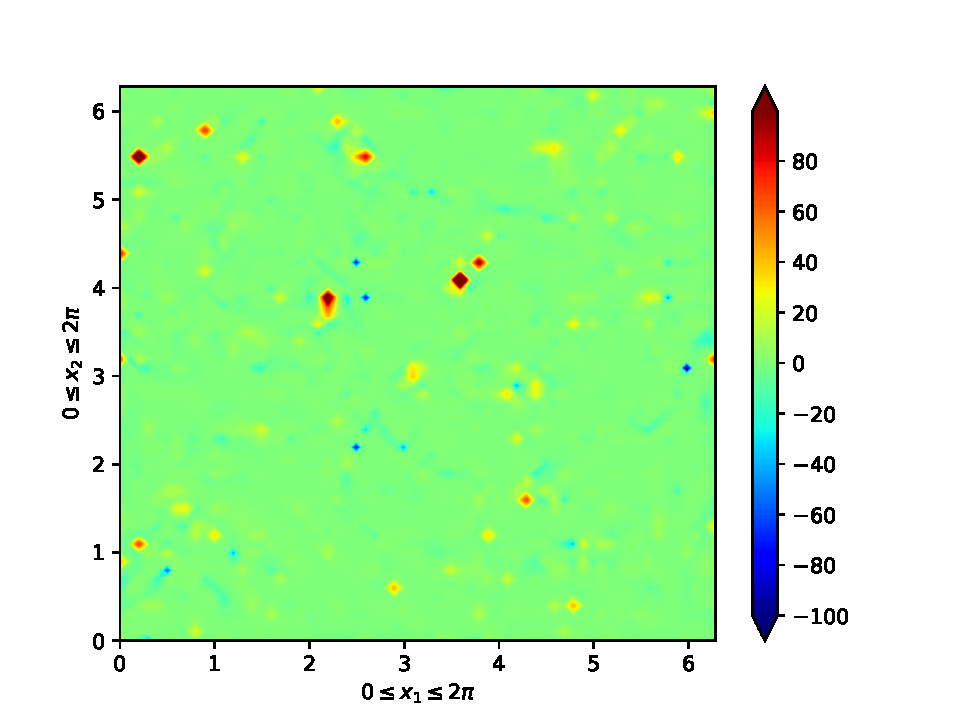
\includegraphics[height=1.75in]{media/run-cds-65/Pi-enst-1310}
        \caption{$\Pi_{\Omega}$}
    \end{subfigure}
    \newline
    \begin{subfigure}{0.45\textwidth}
        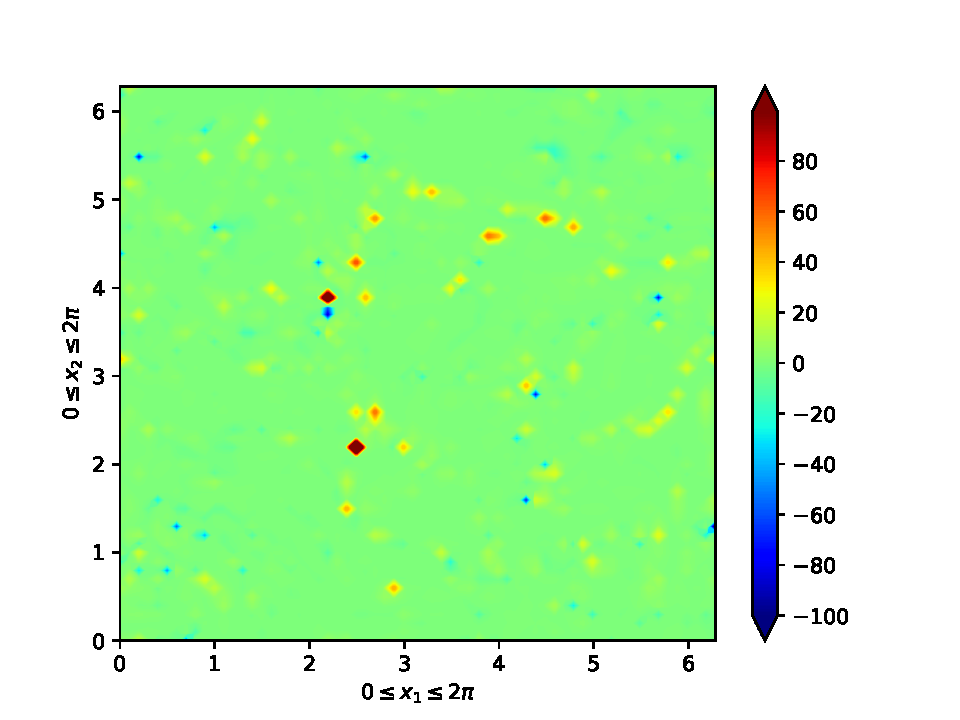
\includegraphics[height=1.75in]{media/run-cds-65/P-enst-1310}
        \caption{$P_{\Omega}$}
    \end{subfigure}
    ~
    \begin{subfigure}{0.45\textwidth}
        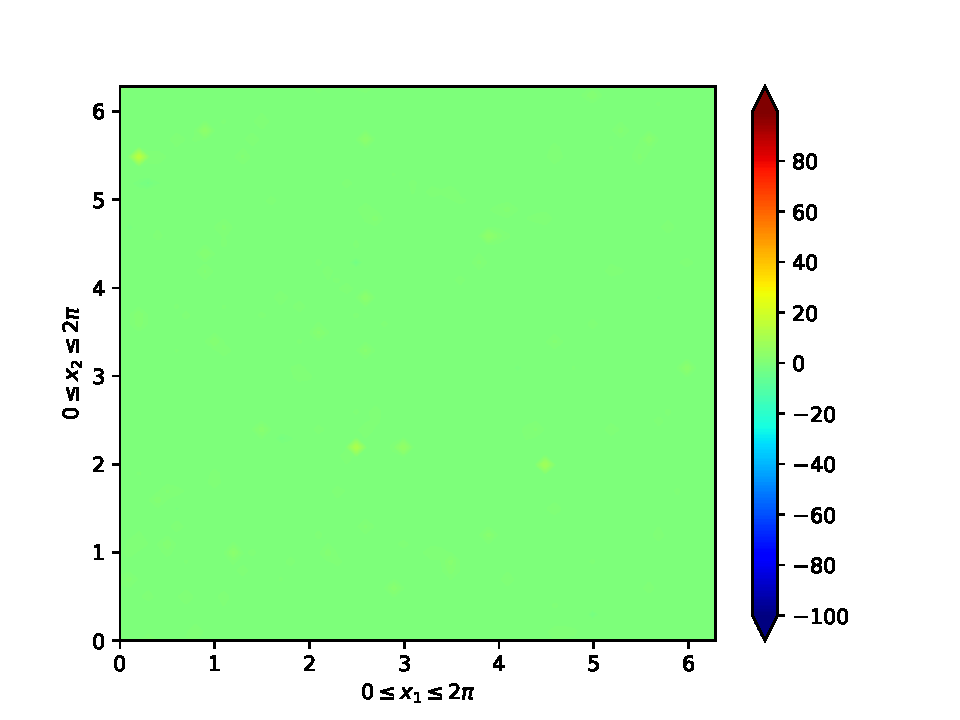
\includegraphics[height=1.75in]{media/run-cds-65/B-enst-1310}
        \caption{$B_{\Omega}$}
    \end{subfigure}
    \newline
    \begin{subfigure}{0.45\textwidth}
        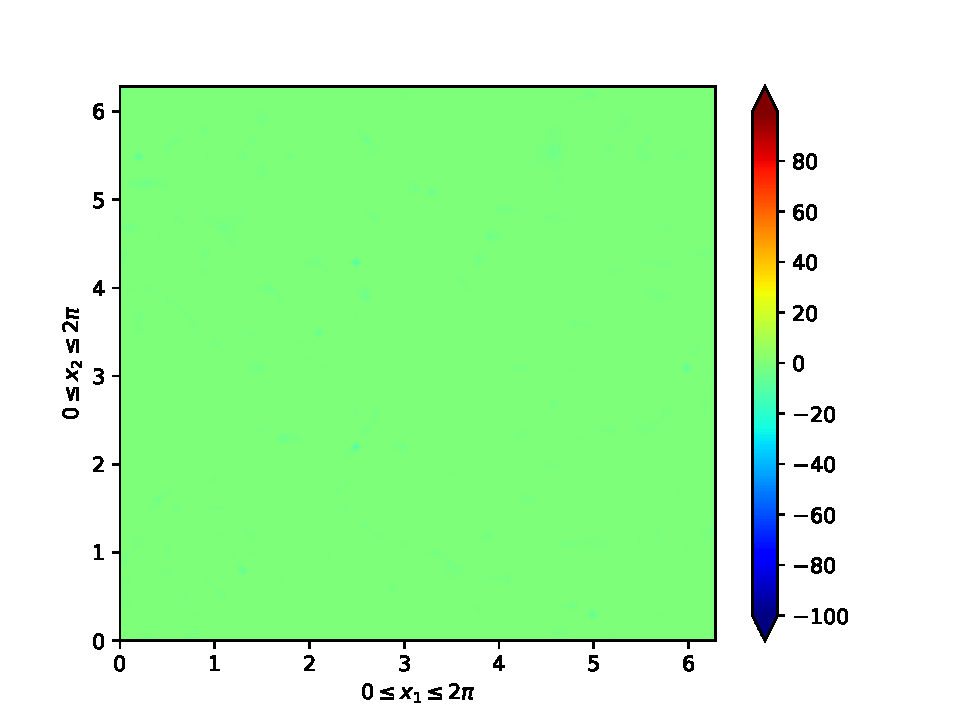
\includegraphics[height=1.75in]{media/run-cds-65/D-enst-1310}
        \caption{$D_{\Omega}$}
    \end{subfigure}
\end{figure}

\newpage

\begin{figure}[H]
    \begin{subfigure}[H]{0.45\textwidth}
        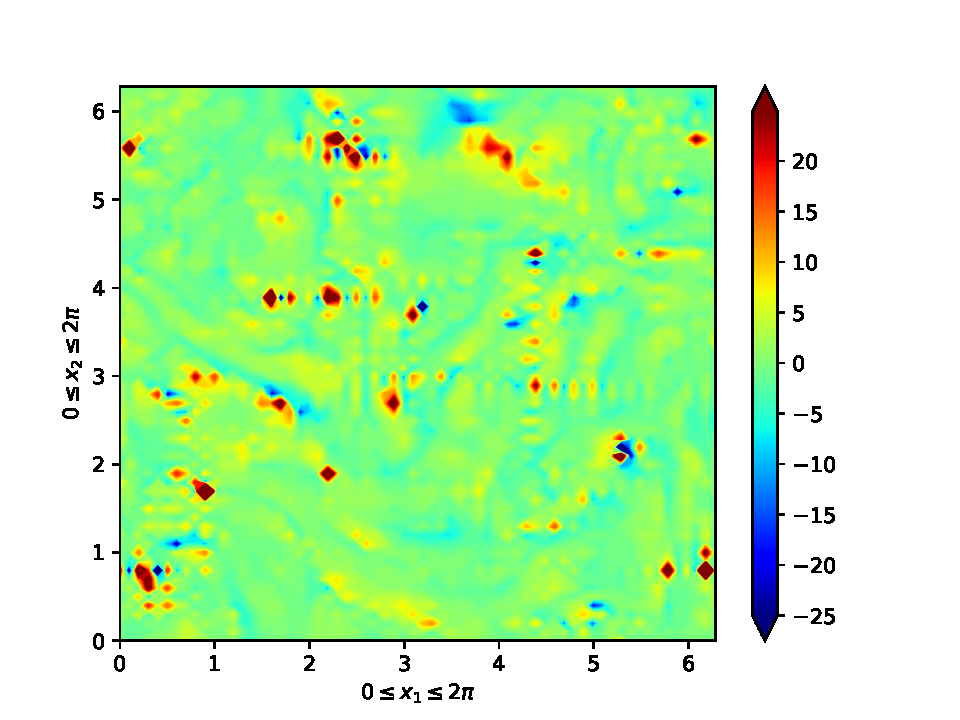
\includegraphics[height=1.75in]{media/run-cds-65/ke-1310}
        \caption{$\frac{1}{k} \frac{D k}{Dt}$}
    \end{subfigure}
    ~
    \begin{subfigure}{0.45\textwidth}
        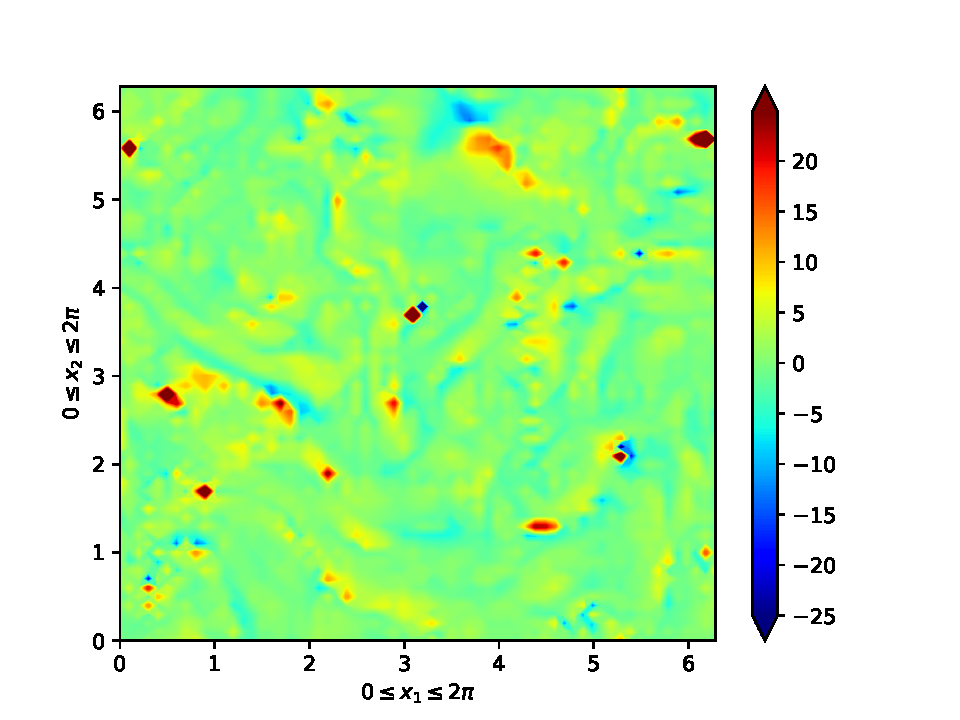
\includegraphics[height=1.75in]{media/run-cds-65/A-ke-1310}
        \caption{$A$}
    \end{subfigure}
    \newline
    \begin{subfigure}{0.45\textwidth}
        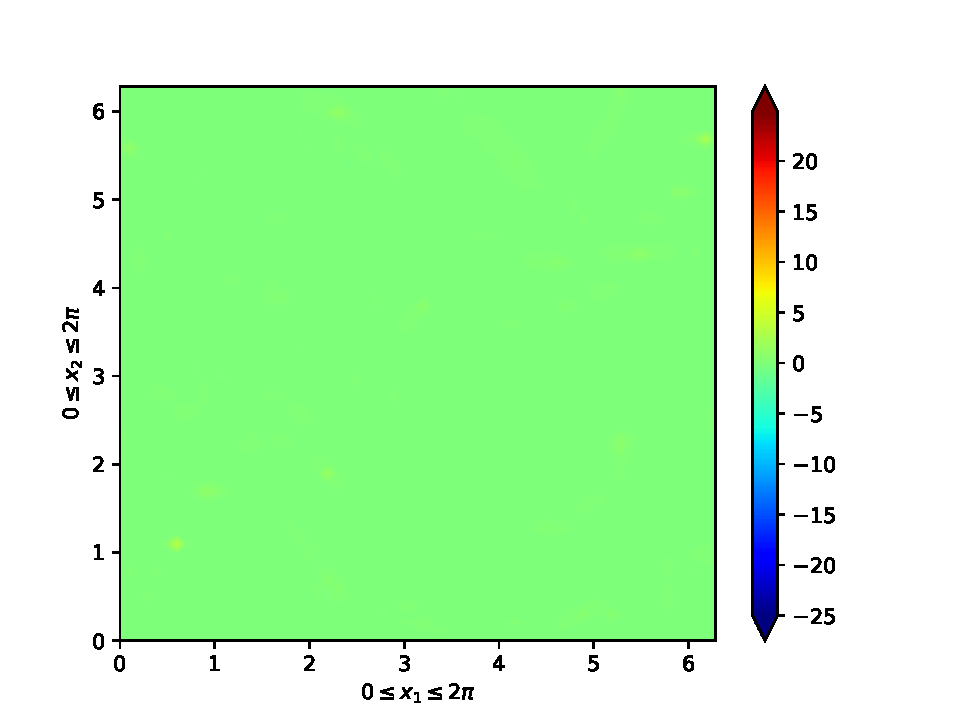
\includegraphics[height=1.75in]{media/run-cds-65/C-ke-1310}
        \caption{$C$}
    \end{subfigure}
    ~
    \begin{subfigure}{0.45\textwidth}
        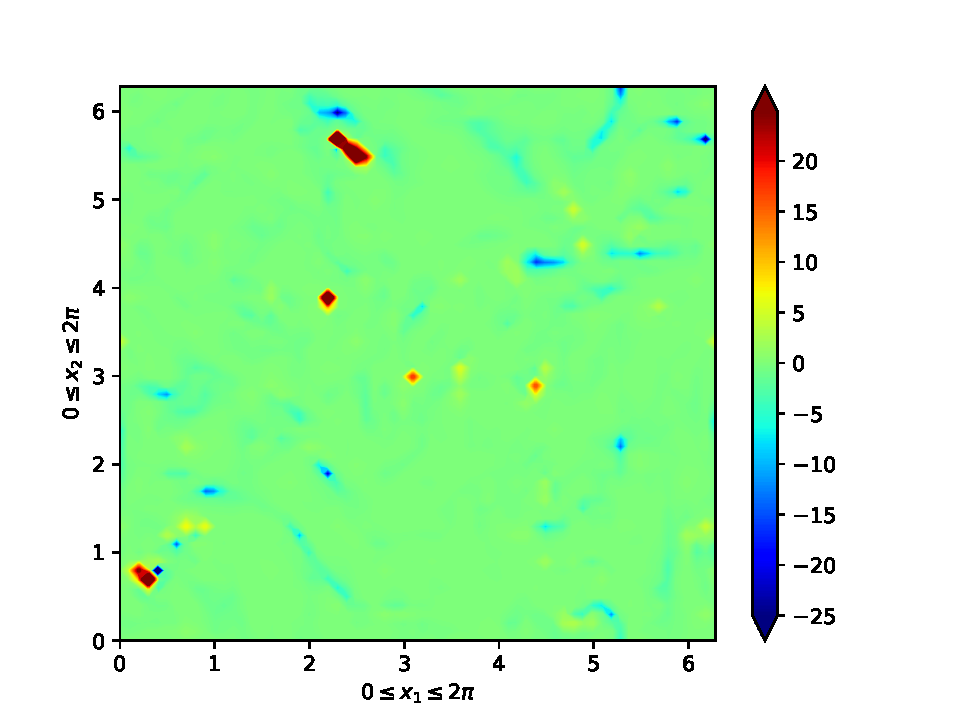
\includegraphics[height=1.75in]{media/run-cds-65/P-ke-1310}
        \caption{$P$}
    \end{subfigure}
    \newline
    \begin{subfigure}{0.45\textwidth}
        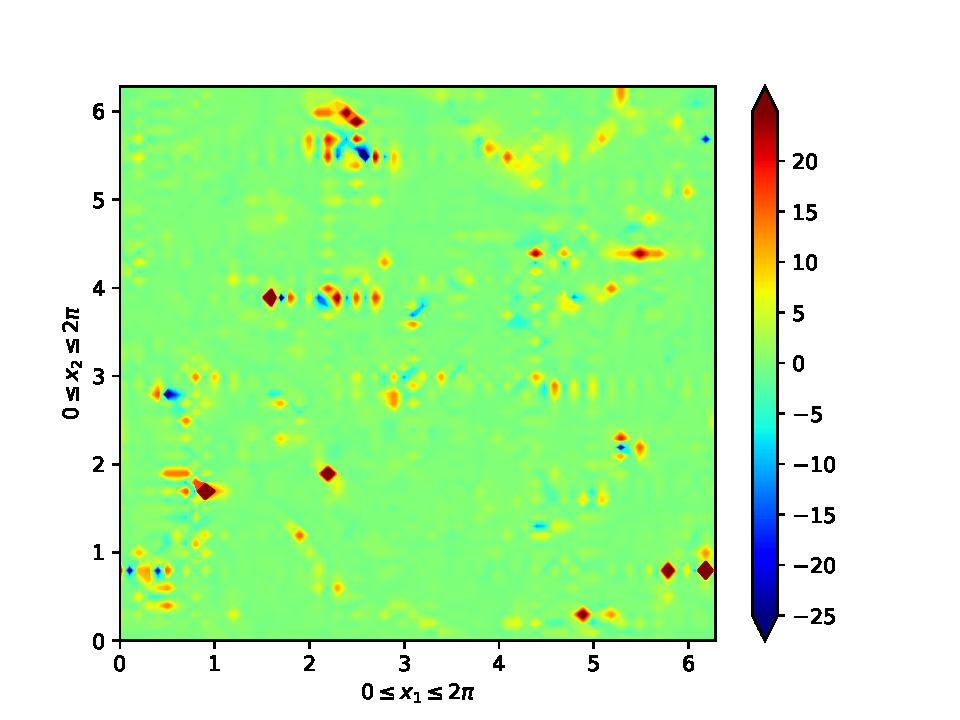
\includegraphics[height=1.75in]{media/run-cds-65/B-ke-1310}
        \caption{$B$}
    \end{subfigure}
    ~
    \begin{subfigure}{0.45\textwidth}
        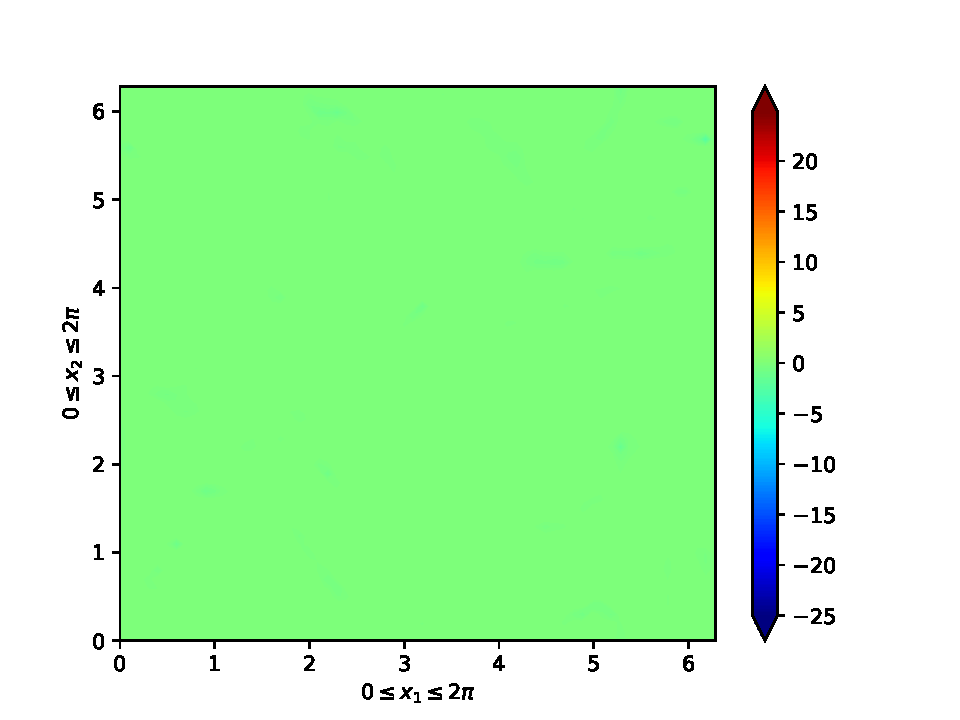
\includegraphics[height=1.75in]{media/run-cds-65/D-ke-1310}
        \caption{$D$}
    \end{subfigure}
\end{figure}

\newpage
%------------------------------------------------------------------------------%
% 1318                                                                         %
%------------------------------------------------------------------------------%
\subsubsection{$t=29.99$ i.e., $t=t^{\ast} - \Delta t$} 
\begin{figure}[H]
    \begin{subfigure}[H]{0.45\textwidth}
        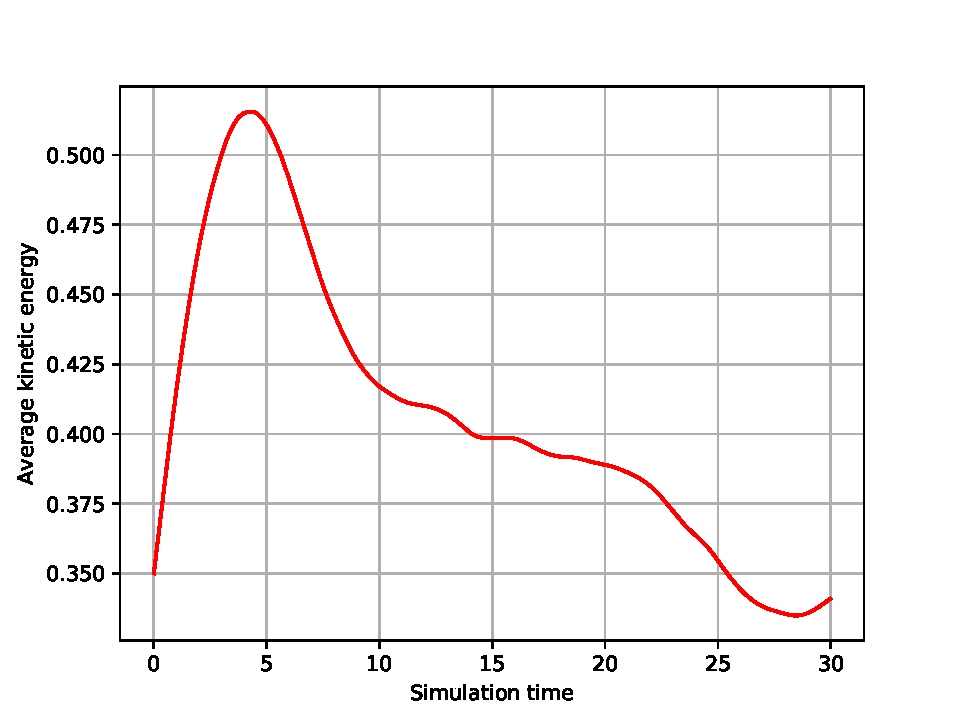
\includegraphics[height=1.75in]{media/run-cds-65/ke-average1318}
        \caption{Average kinetic energy}
    \end{subfigure}
    ~
    \begin{subfigure}[H]{0.45\textwidth}
        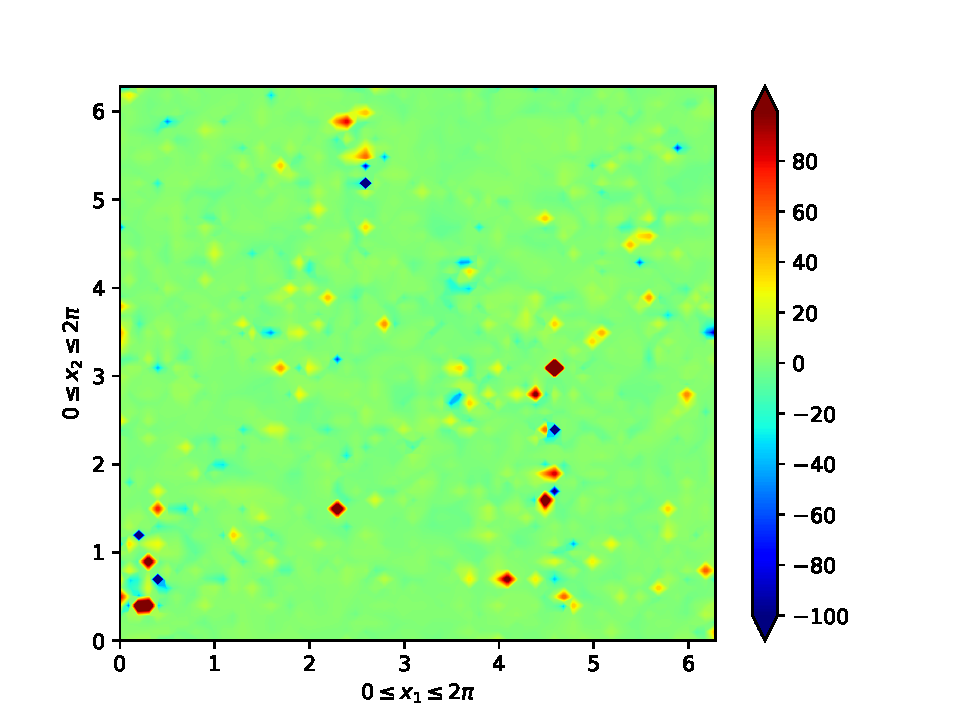
\includegraphics[height=1.75in]{media/run-cds-65/enst-1318}
        \caption{$\frac{1}{\Omega} \frac{D \Omega}{Dt}$}
    \end{subfigure}
    \newline
    \begin{subfigure}{0.45\textwidth}
        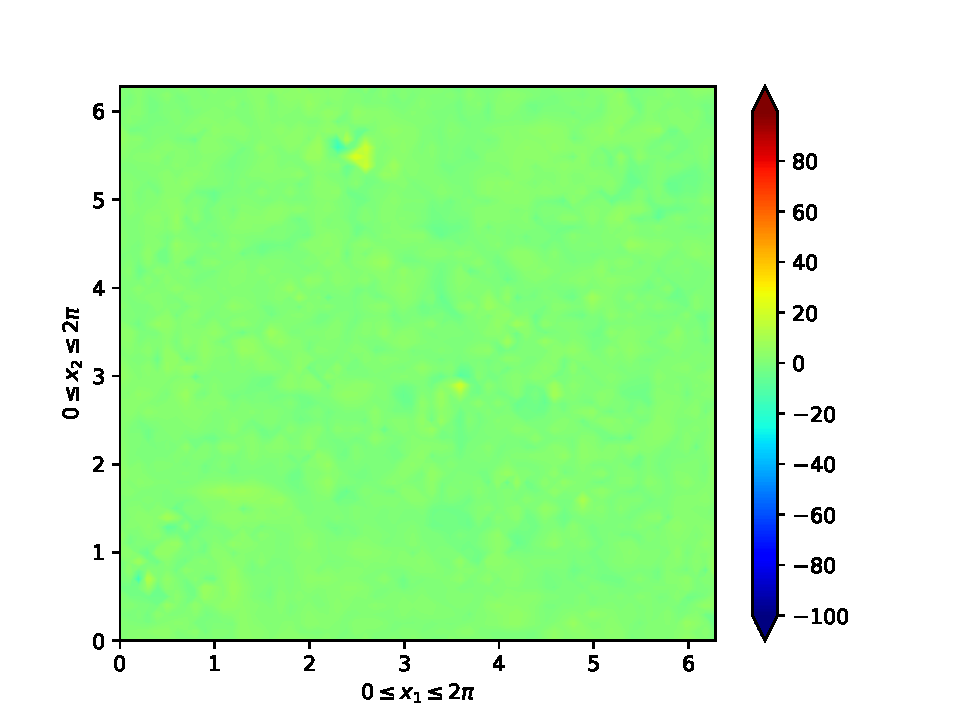
\includegraphics[height=1.75in]{media/run-cds-65/A-enst-1318}
        \caption{$A_{\Omega}$}
    \end{subfigure}
    ~
    \begin{subfigure}{0.45\textwidth}
        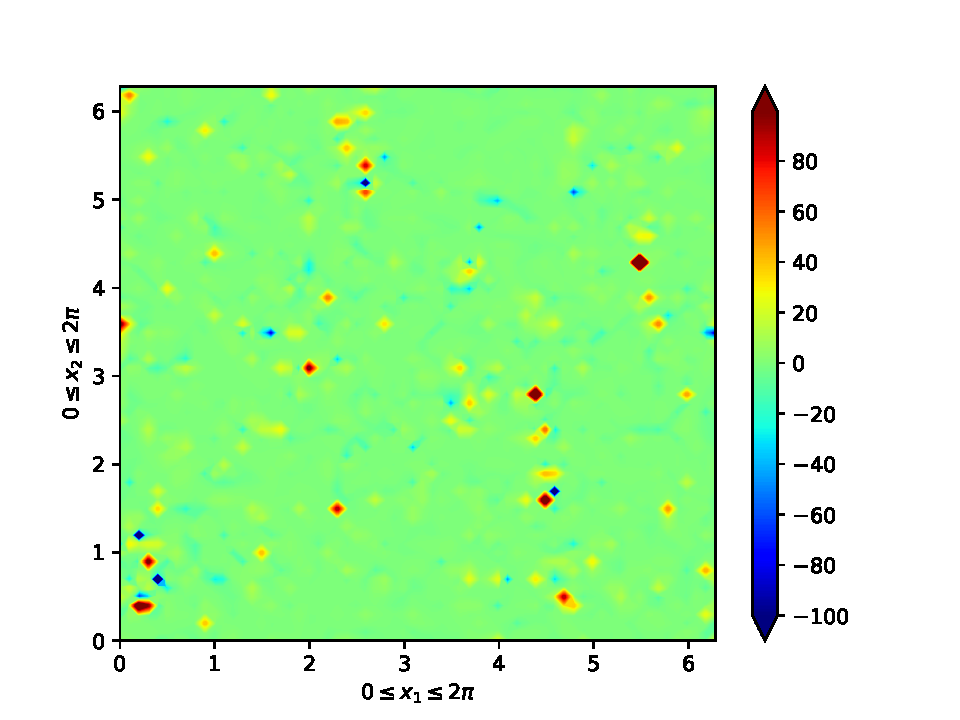
\includegraphics[height=1.75in]{media/run-cds-65/Pi-enst-1318}
        \caption{$\Pi_{\Omega}$}
    \end{subfigure}
    \newline
    \begin{subfigure}{0.45\textwidth}
        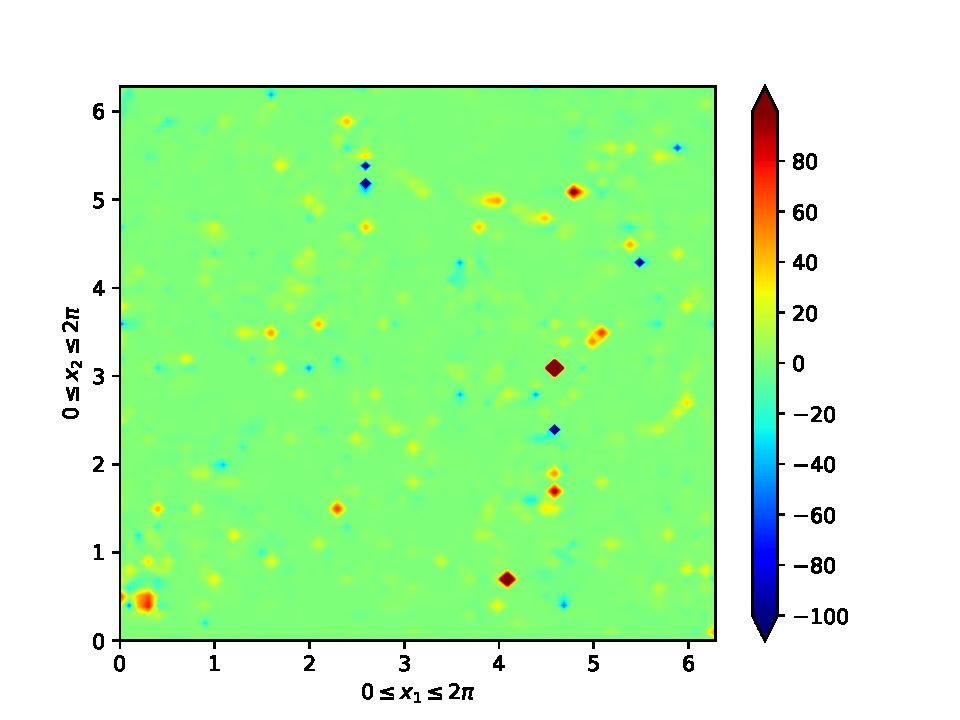
\includegraphics[height=1.75in]{media/run-cds-65/P-enst-1318}
        \caption{$P_{\Omega}$}
    \end{subfigure}
    ~
    \begin{subfigure}{0.45\textwidth}
        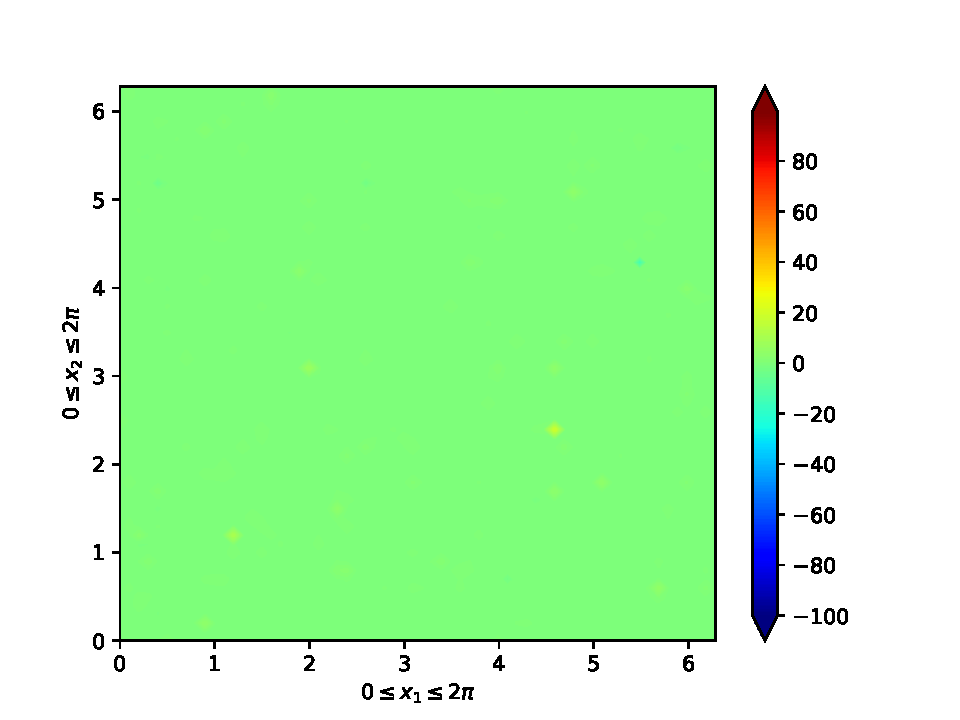
\includegraphics[height=1.75in]{media/run-cds-65/B-enst-1318}
        \caption{$B_{\Omega}$}
    \end{subfigure}
    \newline
    \begin{subfigure}{0.45\textwidth}
        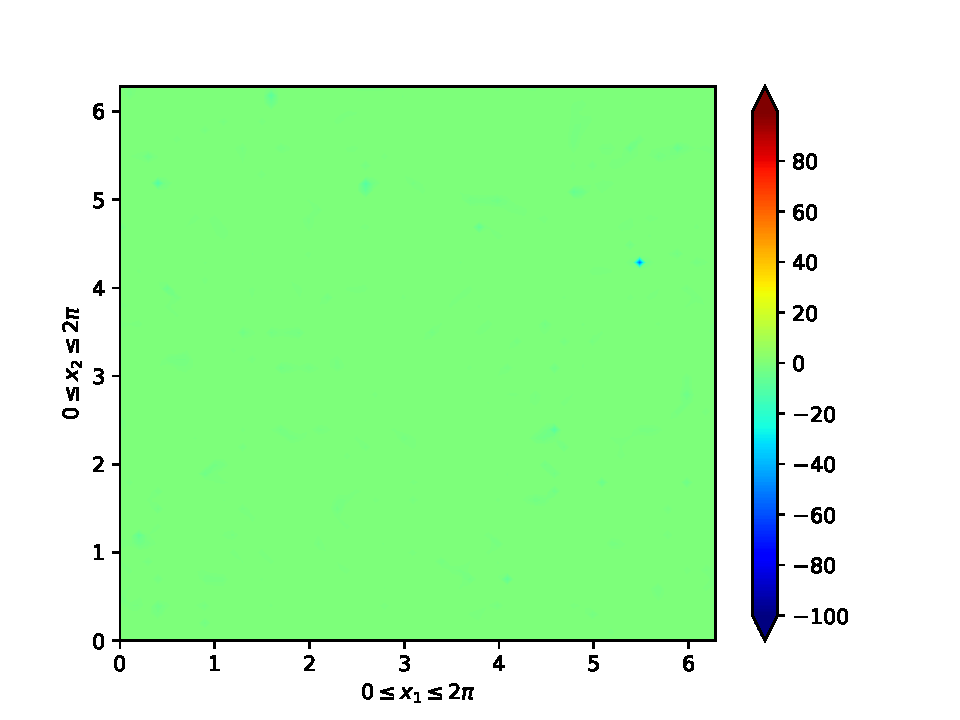
\includegraphics[height=1.75in]{media/run-cds-65/D-enst-1318}
        \caption{$D_{\Omega}$}
    \end{subfigure}
\end{figure}


\newpage

\begin{figure}[H]
    \begin{subfigure}[H]{0.45\textwidth}
        \includegraphics[height=1.75in]{media/run-cds-65/ke-1318}
        \caption{$\frac{1}{k} \frac{D k}{Dt}$}
    \end{subfigure}
    ~
    \begin{subfigure}{0.45\textwidth}
        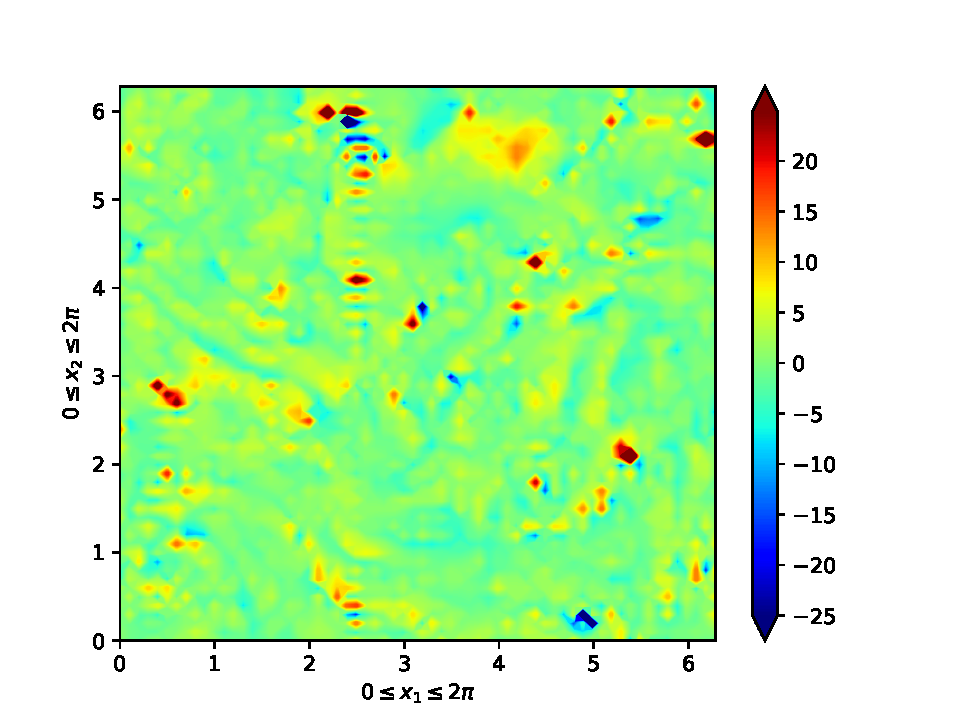
\includegraphics[height=1.75in]{media/run-cds-65/A-ke-1318}
        \caption{$A$}
    \end{subfigure}
    \newline
    \begin{subfigure}{0.45\textwidth}
        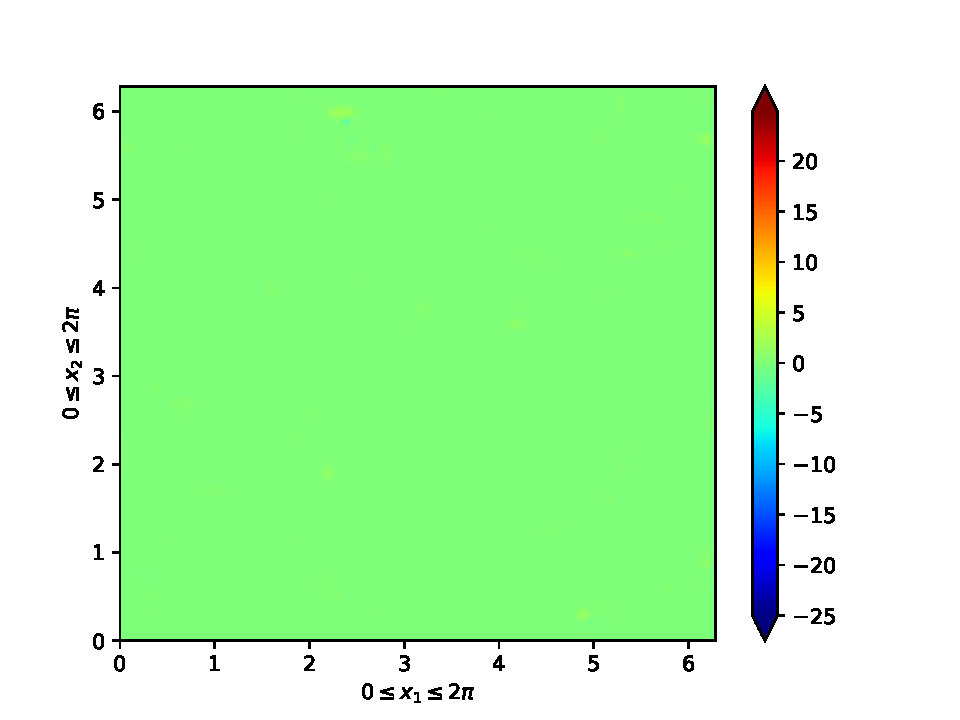
\includegraphics[height=1.75in]{media/run-cds-65/C-ke-1318}
        \caption{$C$}
    \end{subfigure}
    ~
    \begin{subfigure}{0.45\textwidth}
        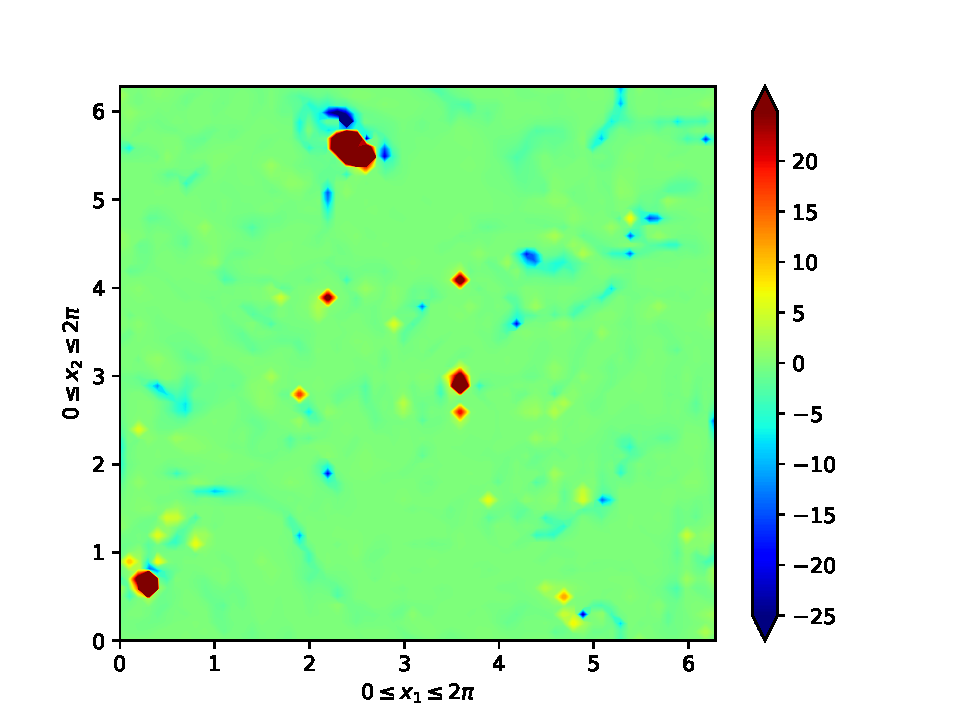
\includegraphics[height=1.75in]{media/run-cds-65/P-ke-1318}
        \caption{$P$}
    \end{subfigure}
    \newline
    \begin{subfigure}{0.45\textwidth}
        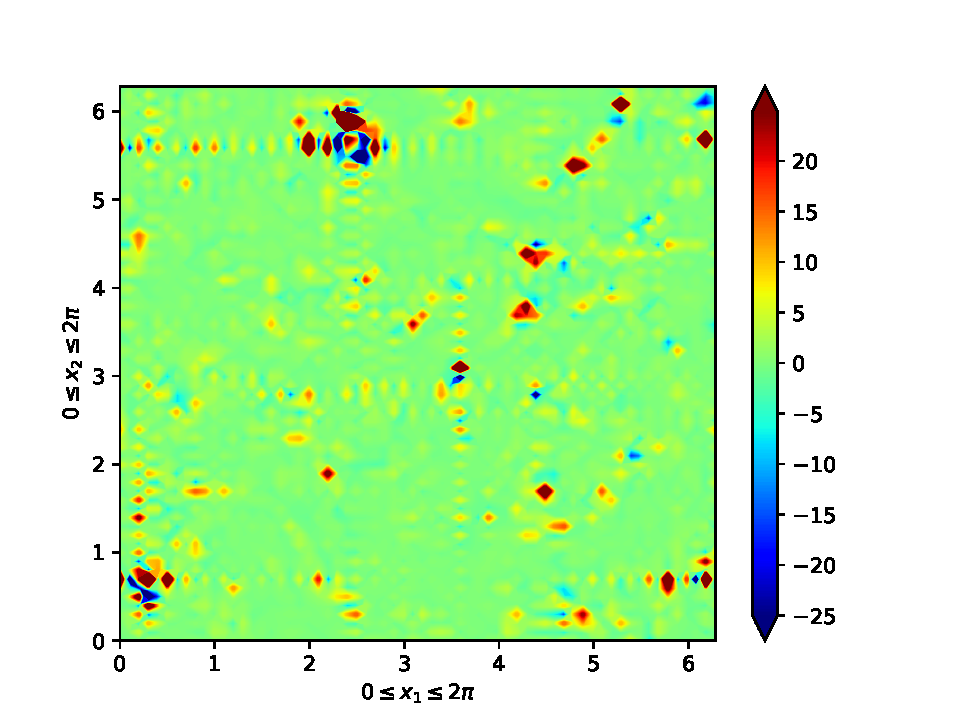
\includegraphics[height=1.75in]{media/run-cds-65/B-ke-1318}
        \caption{$B$}
    \end{subfigure}
    ~
    \begin{subfigure}{0.45\textwidth}
        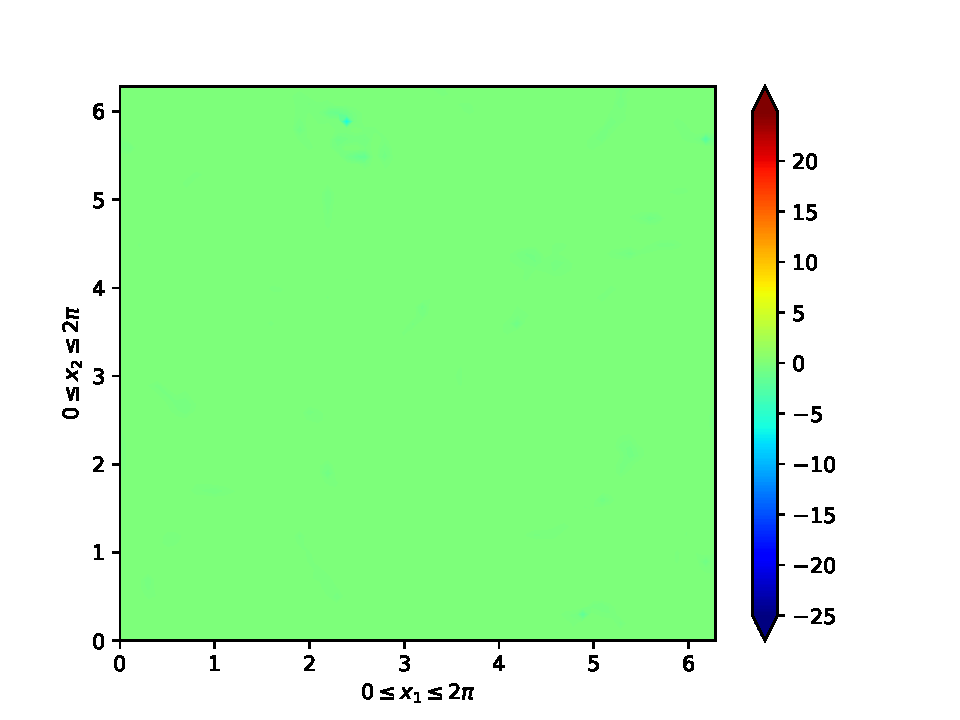
\includegraphics[height=1.75in]{media/run-cds-65/D-ke-1318}
        \caption{$D$}
    \end{subfigure}
\end{figure}

\newpage

%------------------------------------------------------------------------------%
% 1320                                                                         %
%------------------------------------------------------------------------------%
\subsubsection{$t=30.04$ i.e., 1st time step where $C_{DS}=0.65$ is applied} 
\begin{figure}[H]
    \begin{subfigure}[H]{0.45\textwidth}
        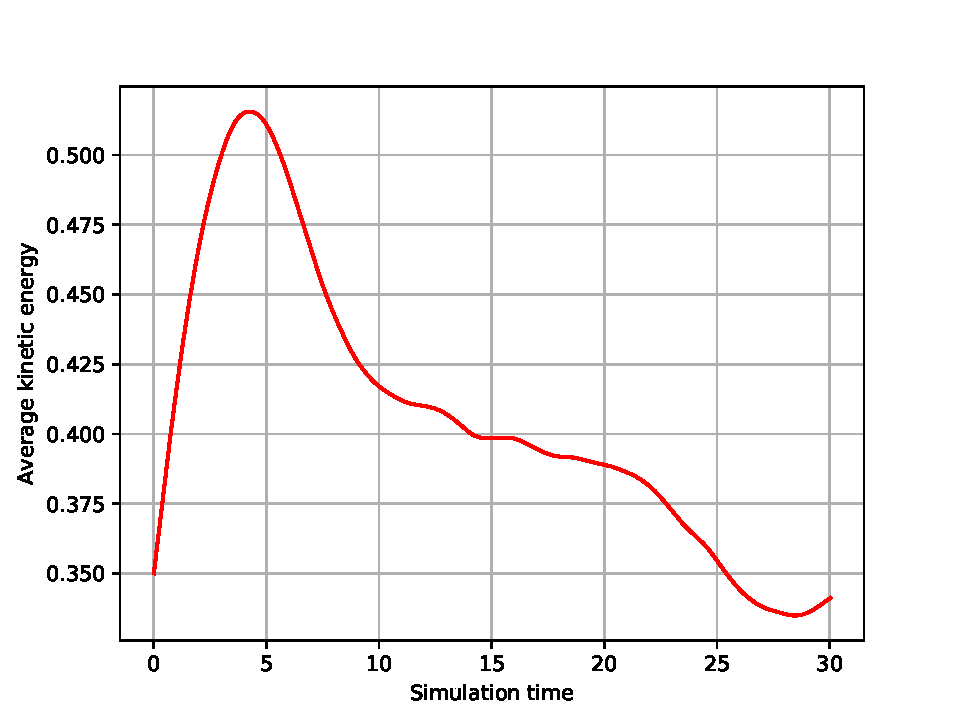
\includegraphics[height=1.75in]{media/run-cds-65/ke-average1320}
        \caption{Average kinetic energy}
    \end{subfigure}
    ~
    \begin{subfigure}[H]{0.45\textwidth}
        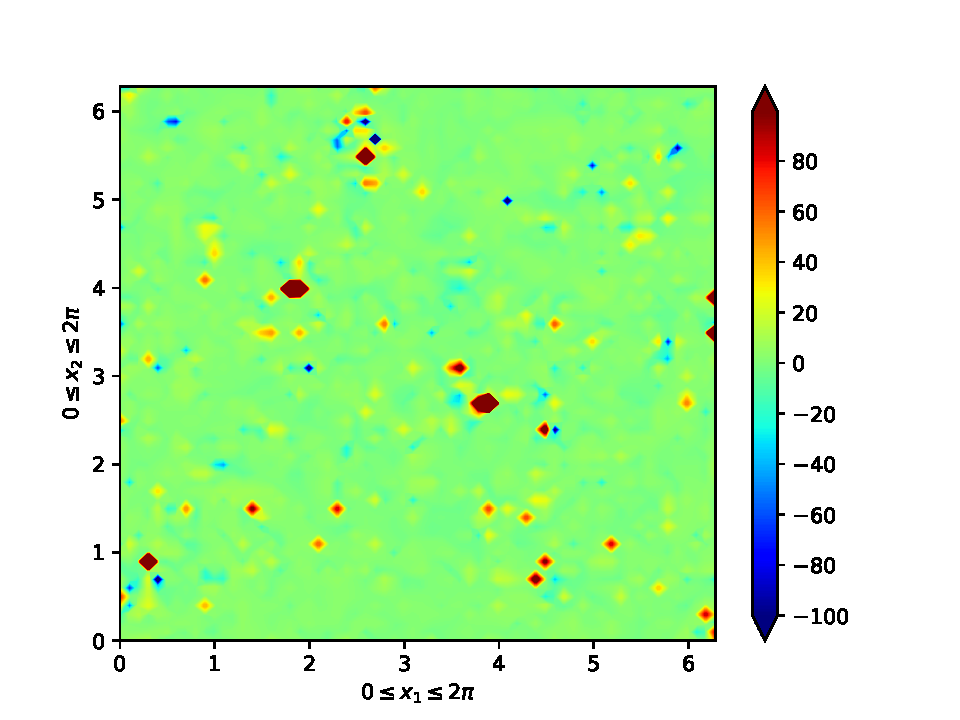
\includegraphics[height=1.75in]{media/run-cds-65/enst-1320}
        \caption{$\frac{1}{\Omega} \frac{D \Omega}{Dt}$}
    \end{subfigure}
    \newline
    \begin{subfigure}{0.45\textwidth}
        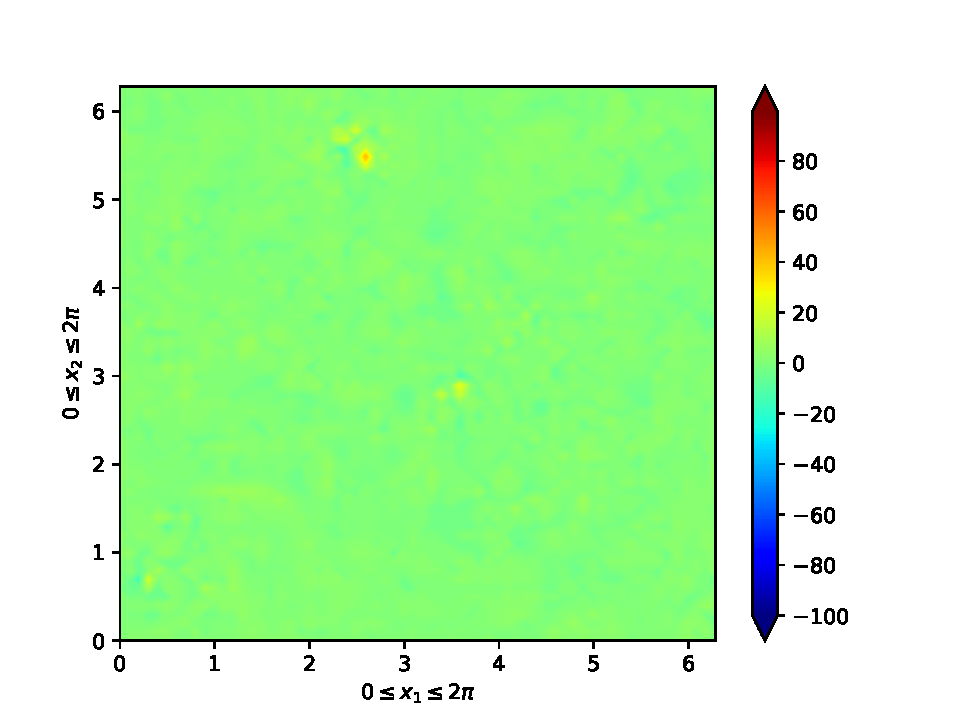
\includegraphics[height=1.75in]{media/run-cds-65/A-enst-1320}
        \caption{$A_{\Omega}$}
    \end{subfigure}
    ~
    \begin{subfigure}{0.45\textwidth}
        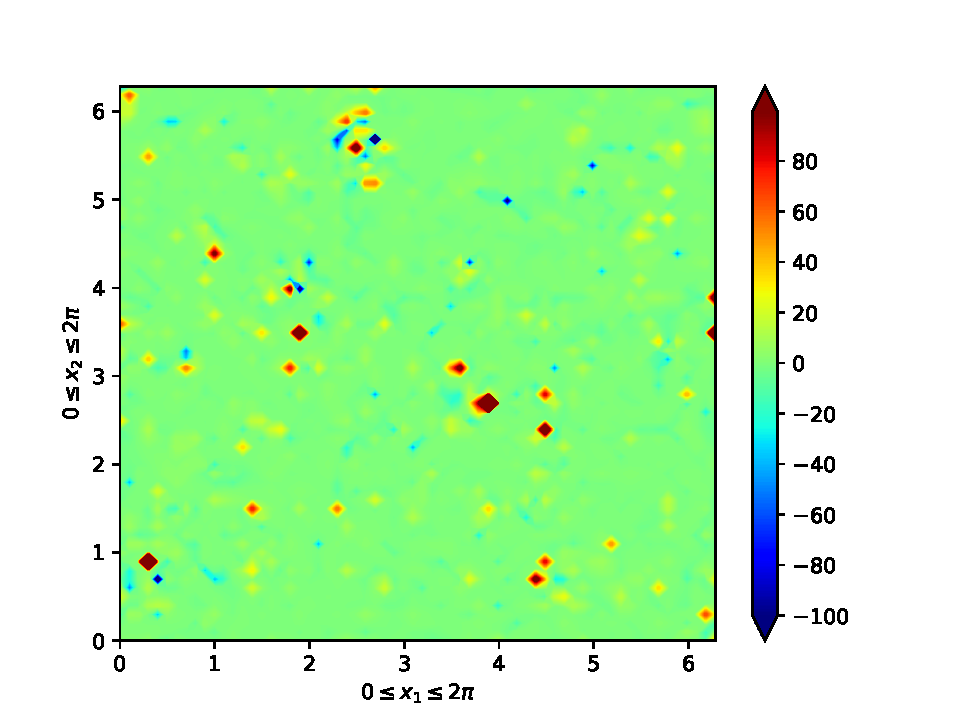
\includegraphics[height=1.75in]{media/run-cds-65/Pi-enst-1320}
        \caption{$\Pi_{\Omega}$}
    \end{subfigure}
    \newline
    \begin{subfigure}{0.45\textwidth}
        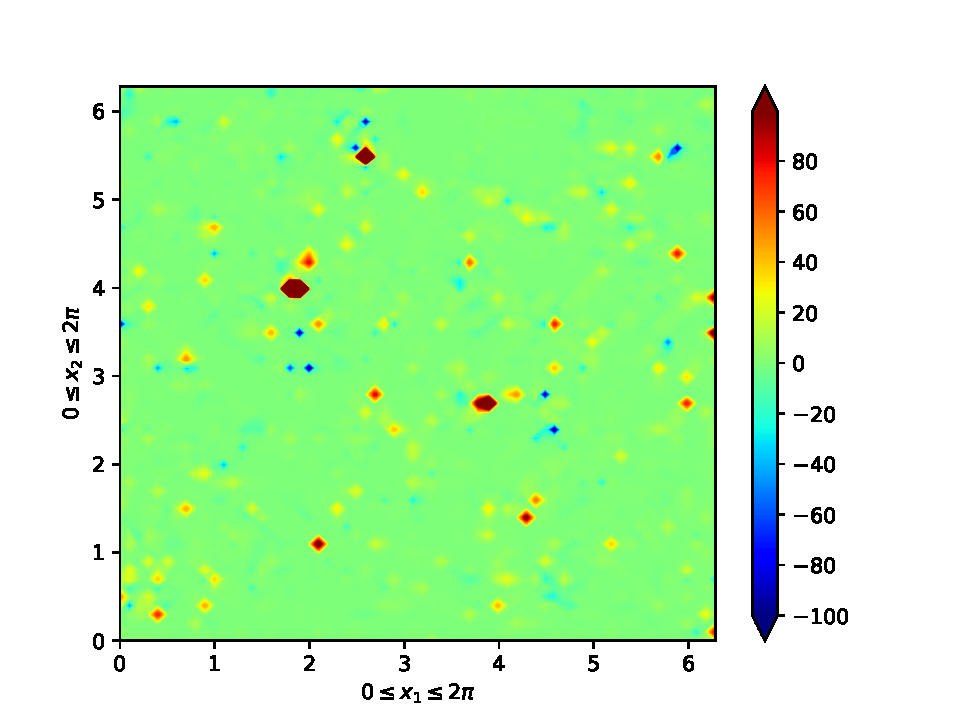
\includegraphics[height=1.75in]{media/run-cds-65/P-enst-1320}
        \caption{$P_{\Omega}$}
    \end{subfigure}
    ~
    \begin{subfigure}{0.45\textwidth}
        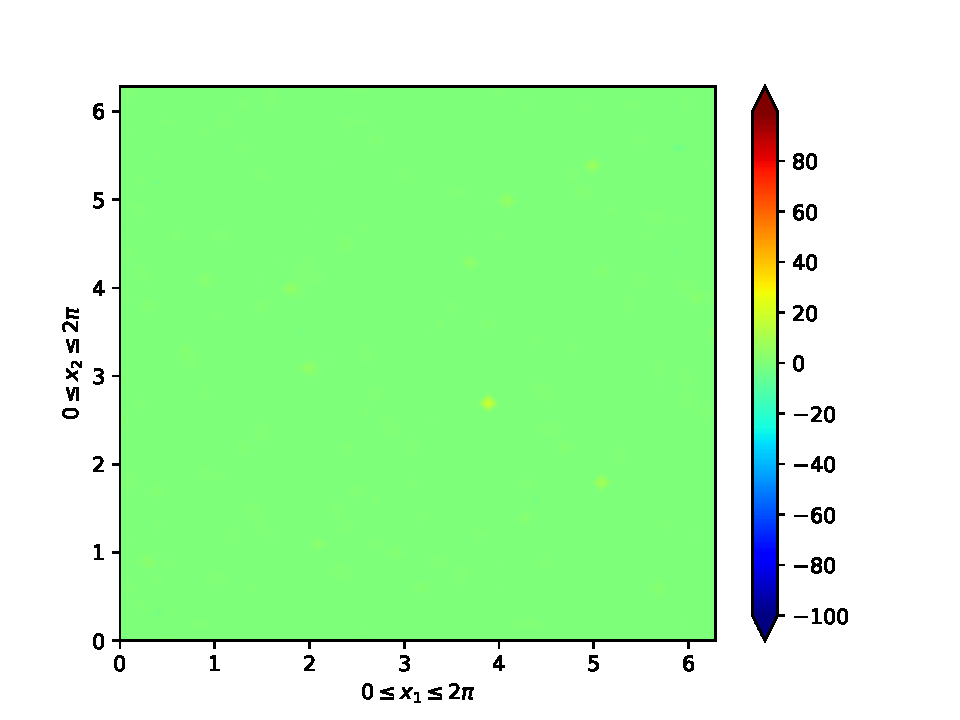
\includegraphics[height=1.75in]{media/run-cds-65/B-enst-1320}
        \caption{$B_{\Omega}$}
    \end{subfigure}
    \newline
    \begin{subfigure}{0.45\textwidth}
        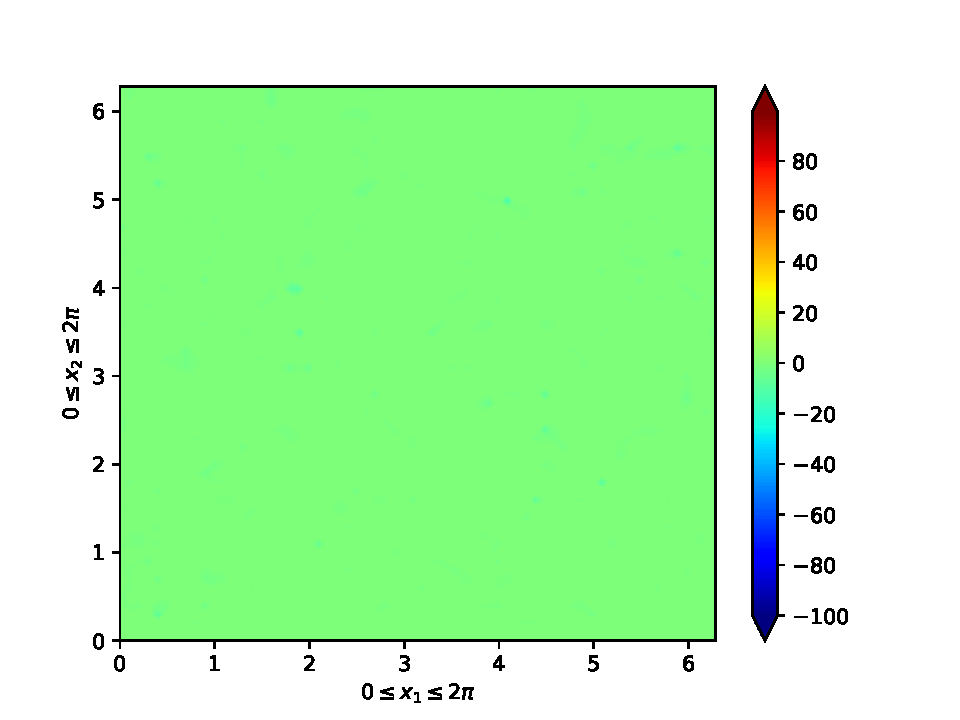
\includegraphics[height=1.75in]{media/run-cds-65/D-enst-1320}
        \caption{$D_{\Omega}$}
    \end{subfigure}
\end{figure}

\newpage

\begin{figure}[H]
    \begin{subfigure}[H]{0.45\textwidth}
        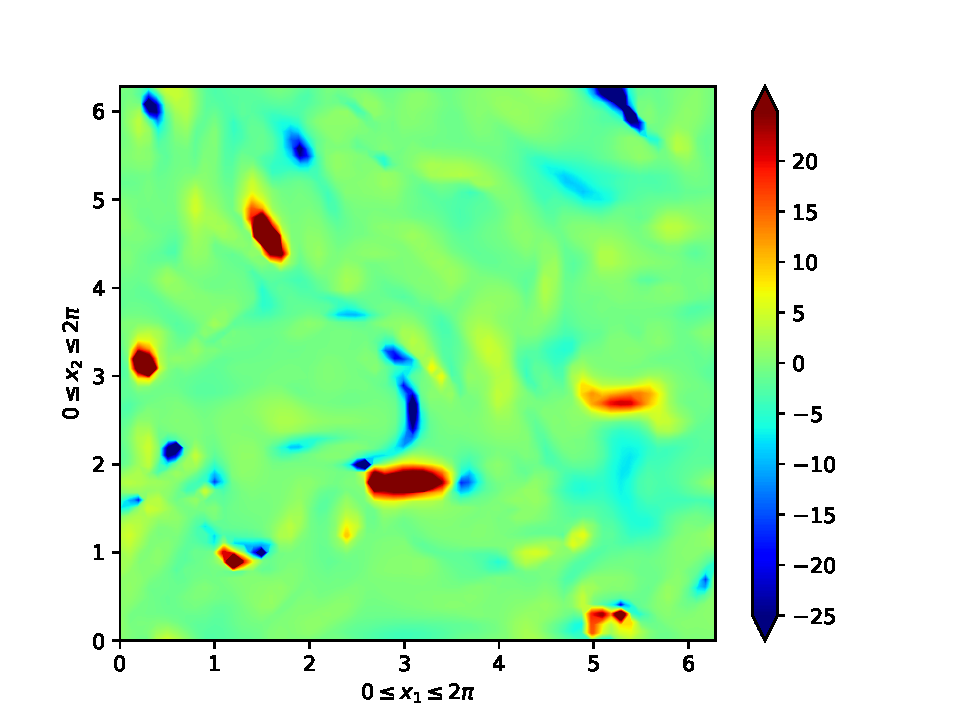
\includegraphics[height=1.75in]{media/run-cds-65/ke-1320}
        \caption{$\frac{1}{k} \frac{D k}{Dt}$}
    \end{subfigure}
    ~
    \begin{subfigure}{0.45\textwidth}
        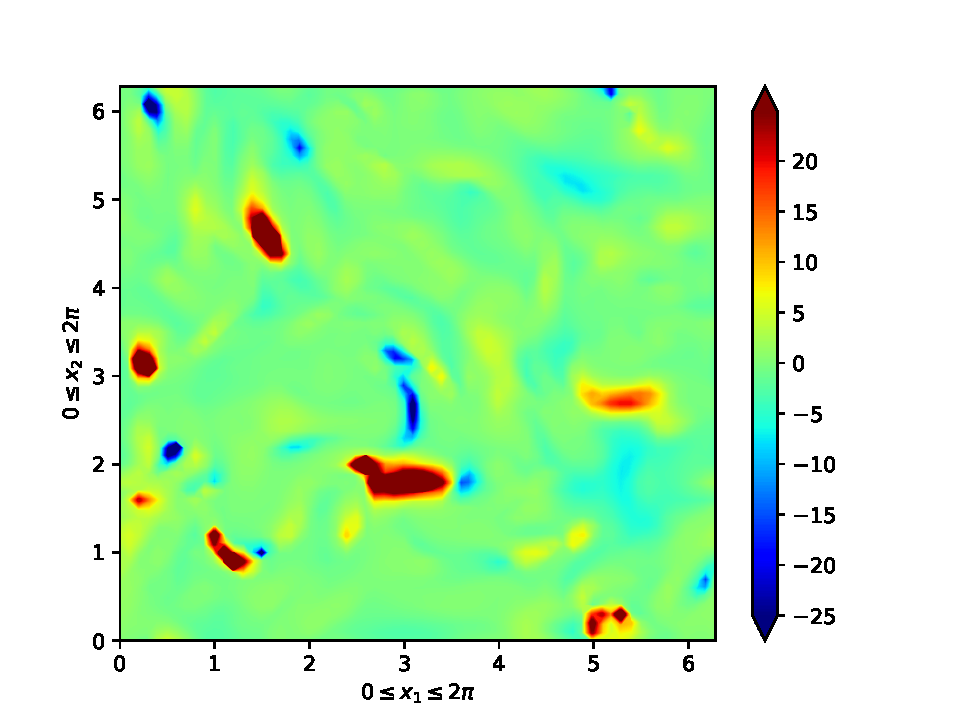
\includegraphics[height=1.75in]{media/run-cds-65/A-ke-1320}
        \caption{$A$}
    \end{subfigure}
    \newline
    \begin{subfigure}{0.45\textwidth}
        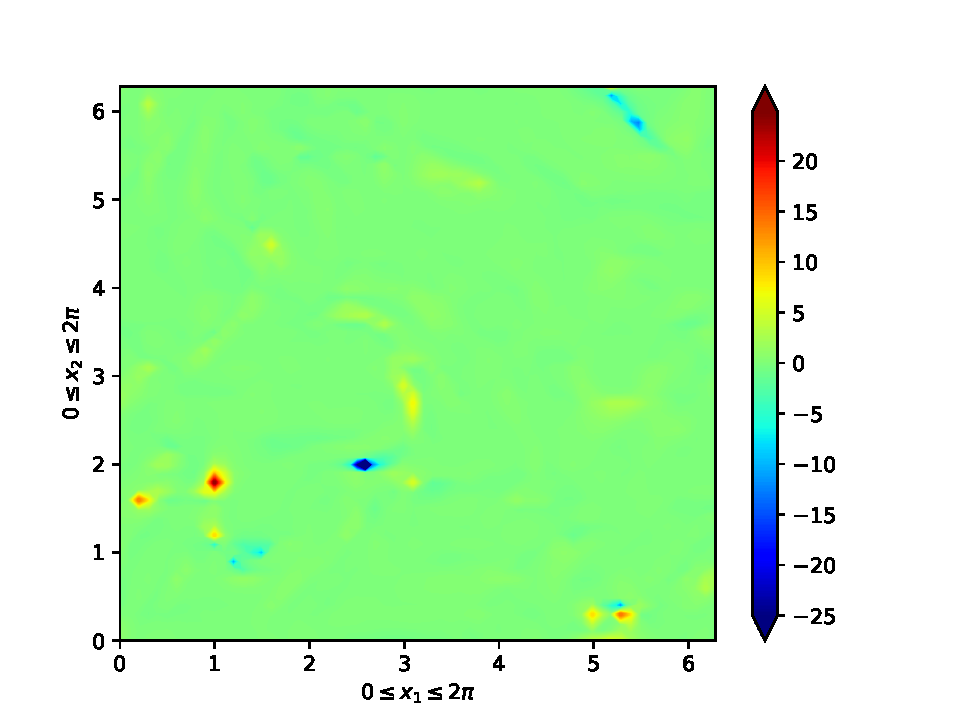
\includegraphics[height=1.75in]{media/run-cds-65/C-ke-1320}
        \caption{$C$}
    \end{subfigure}
    ~
    \begin{subfigure}{0.45\textwidth}
        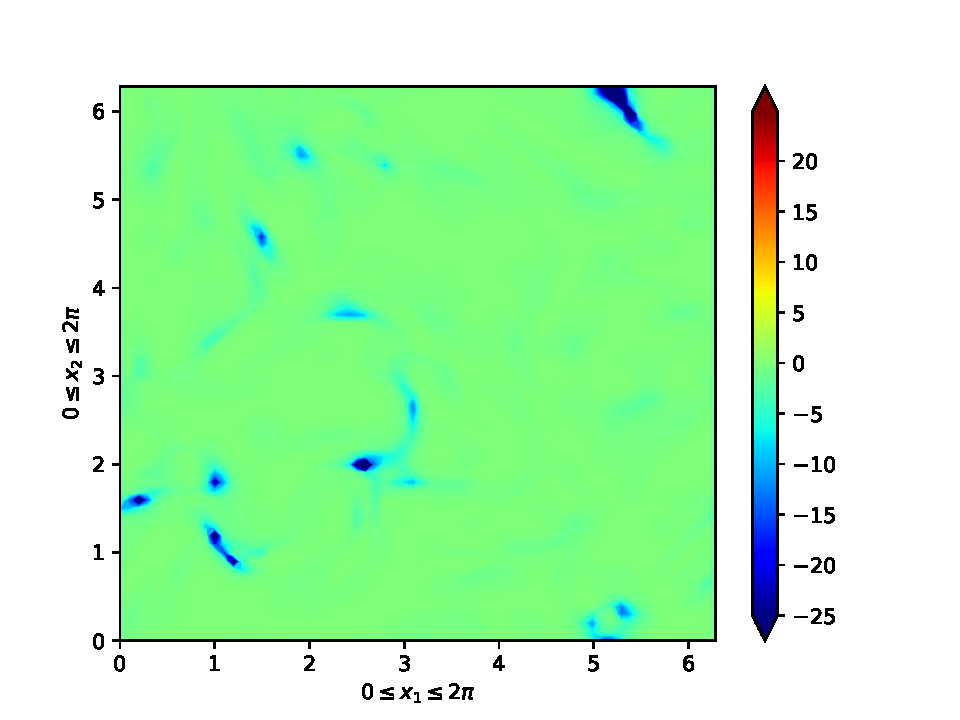
\includegraphics[height=1.75in]{media/run-cds-65/P-ke-1320}
        \caption{$P$}
    \end{subfigure}
    \newline
    \begin{subfigure}{0.45\textwidth}
        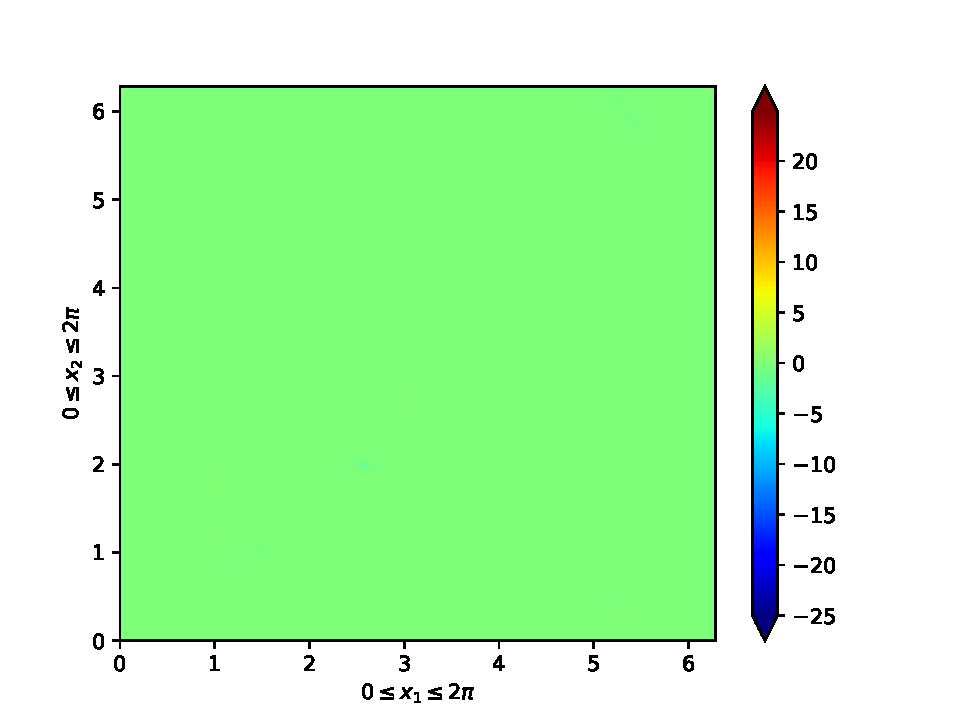
\includegraphics[height=1.75in]{media/run-cds-65/B-ke-1320}
        \caption{$B$}
    \end{subfigure}
    ~
    \begin{subfigure}{0.45\textwidth}
        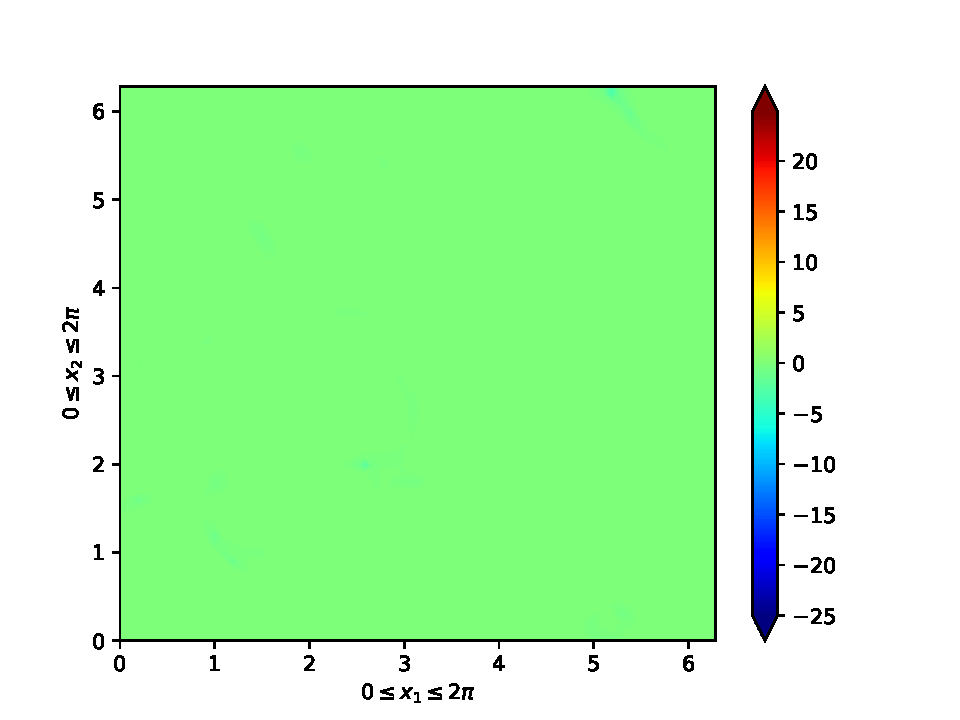
\includegraphics[height=1.75in]{media/run-cds-65/D-ke-1320}
        \caption{$D$}
    \end{subfigure}
\end{figure}

\newpage

%------------------------------------------------------------------------------%
% 1320                                                                         %
%------------------------------------------------------------------------------%
\subsubsection{$t=30.67$ i.e., $t=20\Delta t + t^{\ast}$}
\begin{figure}[H]
    \begin{subfigure}[H]{0.45\textwidth}
        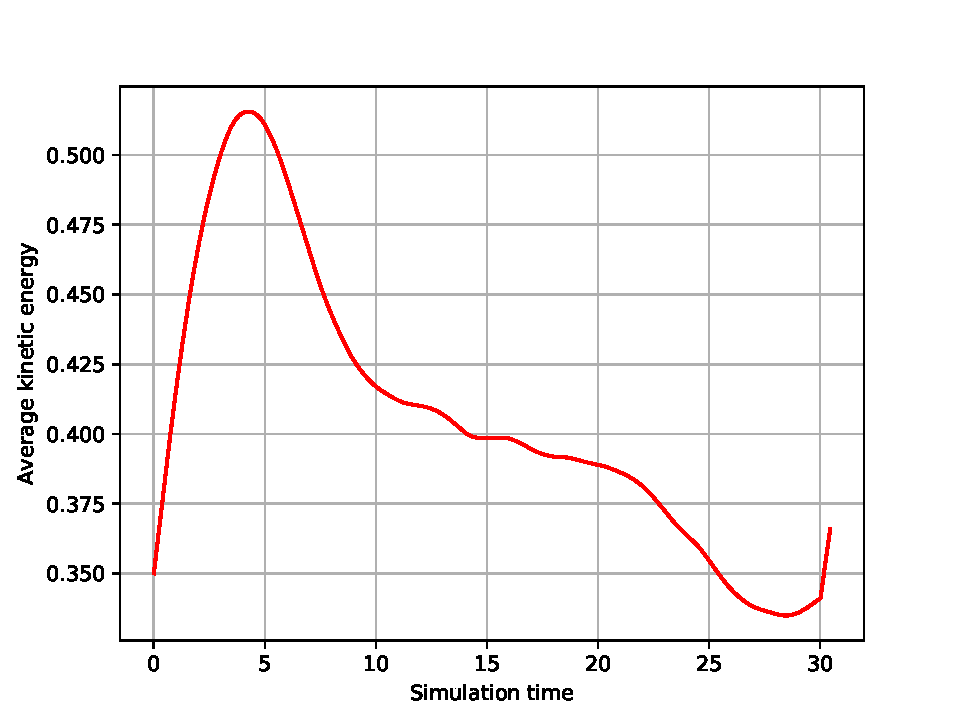
\includegraphics[height=1.75in]{media/run-cds-65/ke-average1340}
        \caption{Average kinetic energy}
    \end{subfigure}
    ~
    \begin{subfigure}[H]{0.45\textwidth}
        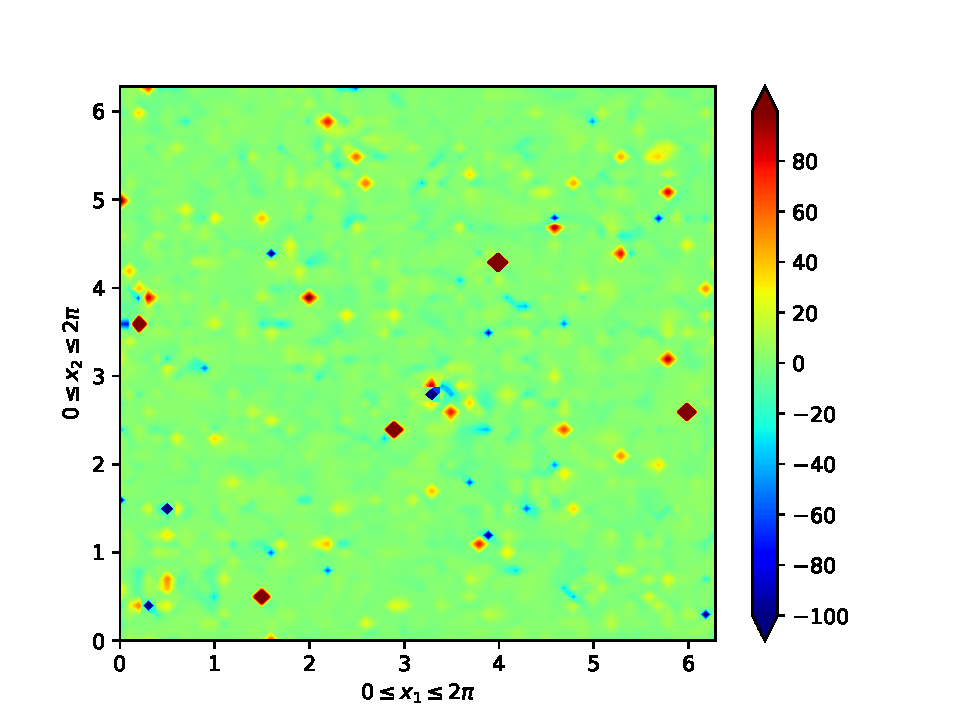
\includegraphics[height=1.75in]{media/run-cds-65/enst-1340}
        \caption{$\frac{1}{\Omega} \frac{D \Omega}{Dt}$}
    \end{subfigure}
    \newline
    \begin{subfigure}{0.45\textwidth}
        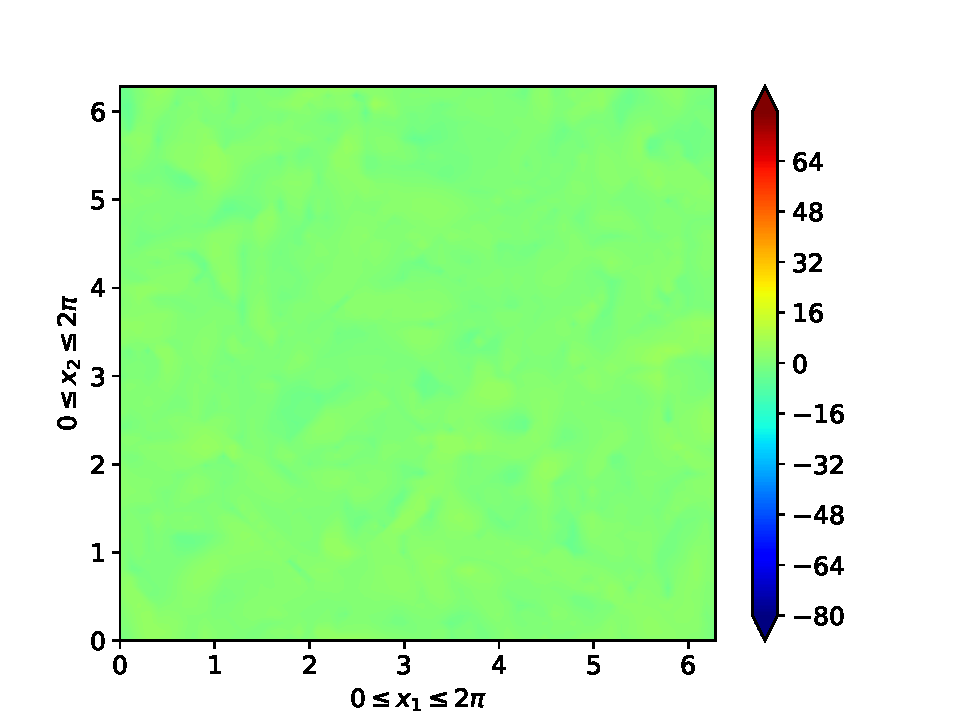
\includegraphics[height=1.75in]{media/run-cds-65/A-enst-1340}
        \caption{$A_{\Omega}$}
    \end{subfigure}
    ~
    \begin{subfigure}{0.45\textwidth}
        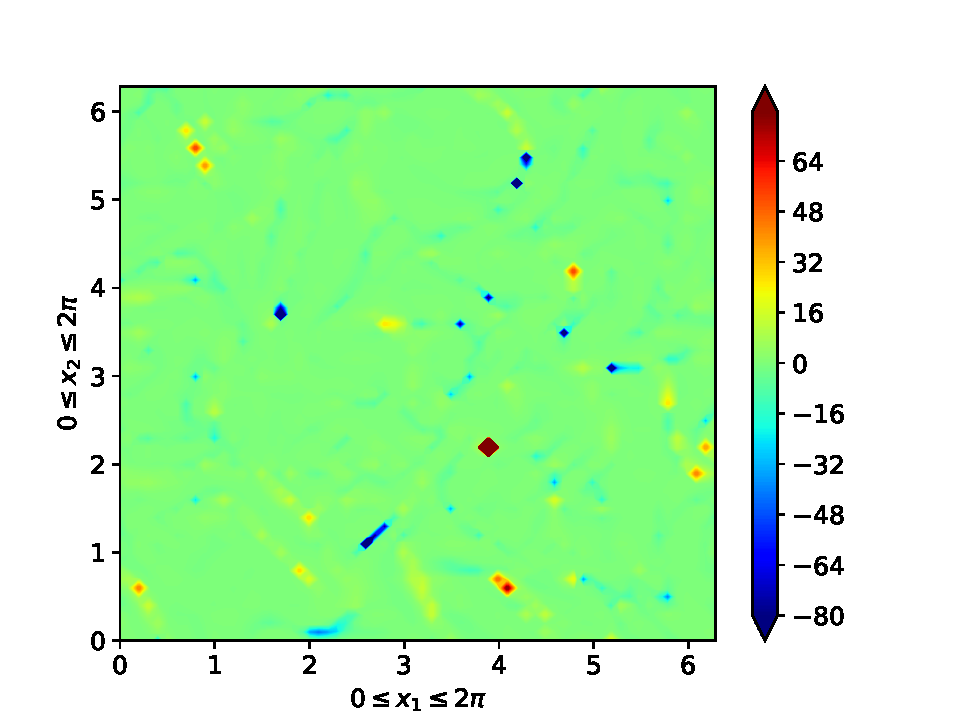
\includegraphics[height=1.75in]{media/run-cds-65/Pi-enst-1340}
        \caption{$\Pi_{\Omega}$}
    \end{subfigure}
    \newline
    \begin{subfigure}{0.45\textwidth}
        \includegraphics[height=1.75in]{media/run-cds-65/P-enst-1340}
        \caption{$P_{\Omega}$}
    \end{subfigure}
    ~
    \begin{subfigure}{0.45\textwidth}
        \includegraphics[height=1.75in]{media/run-cds-65/B-enst-1340}
        \caption{$B_{\Omega}$}
    \end{subfigure}
    \newline
    \begin{subfigure}{0.45\textwidth}
        \includegraphics[height=1.75in]{media/run-cds-65/D-enst-1340}
        \caption{$D_{\Omega}$}
    \end{subfigure}
\end{figure}

\newpage

\begin{figure}[H]
    \begin{subfigure}[H]{0.45\textwidth}
        \includegraphics[height=1.75in]{media/run-cds-65/ke-1340}
        \caption{$\frac{1}{k} \frac{D k}{Dt}$}
    \end{subfigure}
    ~
    \begin{subfigure}{0.45\textwidth}
        \includegraphics[height=1.75in]{media/run-cds-65/A-ke-1340}
        \caption{$A$}
    \end{subfigure}
    \newline
    \begin{subfigure}{0.45\textwidth}
        \includegraphics[height=1.75in]{media/run-cds-65/C-ke-1340}
        \caption{$C$}
    \end{subfigure}
    ~
    \begin{subfigure}{0.45\textwidth}
        \includegraphics[height=1.75in]{media/run-cds-65/P-ke-1340}
        \caption{$P$}
    \end{subfigure}
    \newline
    \begin{subfigure}{0.45\textwidth}
        \includegraphics[height=1.75in]{media/run-cds-65/B-ke-1340}
        \caption{$B$}
    \end{subfigure}
    ~
    \begin{subfigure}{0.45\textwidth}
        \includegraphics[height=1.75in]{media/run-cds-65/D-ke-1340}
        \caption{$D$}
    \end{subfigure}
\end{figure}

\newpage

%------------------------------------------------------------------------------%
% 1360                                                                         %
%------------------------------------------------------------------------------%
\subsubsection{$t=30.77$ i.e., $t=40\Delta t + t^{\ast}$}
\begin{figure}[H]
    \begin{subfigure}[H]{0.45\textwidth}
        \includegraphics[height=1.75in]{media/run-cds-65/ke-average1360}
        \caption{Average kinetic energy}
    \end{subfigure}
    ~
    \begin{subfigure}[H]{0.45\textwidth}
        \includegraphics[height=1.75in]{media/run-cds-65/enst-1360}
        \caption{$\frac{1}{\Omega} \frac{D \Omega}{Dt}$}
    \end{subfigure}
    \newline
    \begin{subfigure}{0.45\textwidth}
        \includegraphics[height=1.75in]{media/run-cds-65/A-enst-1360}
        \caption{$A_{\Omega}$}
    \end{subfigure}
    ~
    \begin{subfigure}{0.45\textwidth}
        \includegraphics[height=1.75in]{media/run-cds-65/Pi-enst-1360}
        \caption{$\Pi_{\Omega}$}
    \end{subfigure}
    \newline
    \begin{subfigure}{0.45\textwidth}
        \includegraphics[height=1.75in]{media/run-cds-65/P-enst-1360}
        \caption{$P_{\Omega}$}
    \end{subfigure}
    ~
    \begin{subfigure}{0.45\textwidth}
        \includegraphics[height=1.75in]{media/run-cds-65/B-enst-1360}
        \caption{$B_{\Omega}$}
    \end{subfigure}
    \newline
    \begin{subfigure}{0.45\textwidth}
        \includegraphics[height=1.75in]{media/run-cds-65/D-enst-1360}
        \caption{$D_{\Omega}$}
    \end{subfigure}
\end{figure}

\newpage

\begin{figure}[H]
    \begin{subfigure}[H]{0.45\textwidth}
        \includegraphics[height=1.75in]{media/run-cds-65/ke-1360}
        \caption{$\frac{1}{k} \frac{D k}{Dt}$}
    \end{subfigure}
    ~
    \begin{subfigure}{0.45\textwidth}
        \includegraphics[height=1.75in]{media/run-cds-65/A-ke-1360}
        \caption{$A$}
    \end{subfigure}
    \newline
    \begin{subfigure}{0.45\textwidth}
        \includegraphics[height=1.75in]{media/run-cds-65/C-ke-1360}
        \caption{$C$}
    \end{subfigure}
    ~
    \begin{subfigure}{0.45\textwidth}
        \includegraphics[height=1.75in]{media/run-cds-65/P-ke-1360}
        \caption{$P$}
    \end{subfigure}
    \newline
    \begin{subfigure}{0.45\textwidth}
        \includegraphics[height=1.75in]{media/run-cds-65/B-ke-1360}
        \caption{$B$}
    \end{subfigure}
    ~
    \begin{subfigure}{0.45\textwidth}
        \includegraphics[height=1.75in]{media/run-cds-65/D-ke-1360}
        \caption{$D$}
    \end{subfigure}
\end{figure}

\newpage
%------------------------------------------------------------------------------%
% 1380                                                                         %
%------------------------------------------------------------------------------%
\subsubsection{$t=30.81$ i.e., $t=60\Delta t + t^{\ast}$}
\begin{figure}[H]
    \begin{subfigure}[H]{0.45\textwidth}
        \includegraphics[height=1.75in]{media/run-cds-65/ke-average1380}
        \caption{Average kinetic energy}
    \end{subfigure}
    ~
    \begin{subfigure}[H]{0.45\textwidth}
        \includegraphics[height=1.75in]{media/run-cds-65/enst-1380}
        \caption{$\frac{1}{\Omega} \frac{D \Omega}{Dt}$}
    \end{subfigure}
    \newline
    \begin{subfigure}{0.45\textwidth}
        \includegraphics[height=1.75in]{media/run-cds-65/A-enst-1380}
        \caption{$A_{\Omega}$}
    \end{subfigure}
    ~
    \begin{subfigure}{0.45\textwidth}
        \includegraphics[height=1.75in]{media/run-cds-65/Pi-enst-1380}
        \caption{$\Pi_{\Omega}$}
    \end{subfigure}
    \newline
    \begin{subfigure}{0.45\textwidth}
        \includegraphics[height=1.75in]{media/run-cds-65/P-enst-1380}
        \caption{$P_{\Omega}$}
    \end{subfigure}
    ~
    \begin{subfigure}{0.45\textwidth}
        \includegraphics[height=1.75in]{media/run-cds-65/B-enst-1380}
        \caption{$B_{\Omega}$}
    \end{subfigure}
    \newline
    \begin{subfigure}{0.45\textwidth}
        \includegraphics[height=1.75in]{media/run-cds-65/D-enst-1380}
        \caption{$D_{\Omega}$}
    \end{subfigure}
\end{figure}

\newpage

\begin{figure}[H]
    \begin{subfigure}[H]{0.45\textwidth}
        \includegraphics[height=1.75in]{media/run-cds-65/ke-1380}
        \caption{$\frac{1}{k} \frac{D k}{Dt}$}
    \end{subfigure}
    ~
    \begin{subfigure}{0.45\textwidth}
        \includegraphics[height=1.75in]{media/run-cds-65/A-ke-1380}
        \caption{$A$}
    \end{subfigure}
    \newline
    \begin{subfigure}{0.45\textwidth}
        \includegraphics[height=1.75in]{media/run-cds-65/C-ke-1380}
        \caption{$C$}
    \end{subfigure}
    ~
    \begin{subfigure}{0.45\textwidth}
        \includegraphics[height=1.75in]{media/run-cds-65/P-ke-1380}
        \caption{$P$}
    \end{subfigure}
    \newline
    \begin{subfigure}{0.45\textwidth}
        \includegraphics[height=1.75in]{media/run-cds-65/B-ke-1380}
        \caption{$B$}
    \end{subfigure}
    ~
    \begin{subfigure}{0.45\textwidth}
        \includegraphics[height=1.75in]{media/run-cds-65/D-ke-1380}
        \caption{$D$}
    \end{subfigure}
\end{figure}

\newpage

%------------------------------------------------------------------------------%
% 1400                                                                         %
%------------------------------------------------------------------------------%
\subsubsection{$t=30.84$ i.e., $t=80\Delta t + t^{\ast}$}
\begin{figure}[H]
    \begin{subfigure}[H]{0.45\textwidth}
        \includegraphics[height=1.75in]{media/run-cds-65/ke-average1400}
        \caption{Average kinetic energy}
    \end{subfigure}
    ~
    \begin{subfigure}[H]{0.45\textwidth}
        \includegraphics[height=1.75in]{media/run-cds-65/enst-1400}
        \caption{$\frac{1}{\Omega} \frac{D \Omega}{Dt}$}
    \end{subfigure}
    \newline
    \begin{subfigure}{0.45\textwidth}
        \includegraphics[height=1.75in]{media/run-cds-65/A-enst-1400}
        \caption{$A_{\Omega}$}
    \end{subfigure}
    ~
    \begin{subfigure}{0.45\textwidth}
        \includegraphics[height=1.75in]{media/run-cds-65/Pi-enst-1400}
        \caption{$\Pi_{\Omega}$}
    \end{subfigure}
    \newline
    \begin{subfigure}{0.45\textwidth}
        \includegraphics[height=1.75in]{media/run-cds-65/P-enst-1400}
        \caption{$P_{\Omega}$}
    \end{subfigure}
    ~
    \begin{subfigure}{0.45\textwidth}
        \includegraphics[height=1.75in]{media/run-cds-65/B-enst-1400}
        \caption{$B_{\Omega}$}
    \end{subfigure}
    \newline
    \begin{subfigure}{0.45\textwidth}
        \includegraphics[height=1.75in]{media/run-cds-65/D-enst-1400}
        \caption{$D_{\Omega}$}
    \end{subfigure}
\end{figure}

\newpage

\begin{figure}[H]
    \begin{subfigure}[H]{0.45\textwidth}
        \includegraphics[height=1.75in]{media/run-cds-65/ke-1400}
        \caption{$\frac{1}{k} \frac{D k}{Dt}$}
    \end{subfigure}
    ~
    \begin{subfigure}{0.45\textwidth}
        \includegraphics[height=1.75in]{media/run-cds-65/A-ke-1400}
        \caption{$A$}
    \end{subfigure}
    \newline
    \begin{subfigure}{0.45\textwidth}
        \includegraphics[height=1.75in]{media/run-cds-65/C-ke-1400}
        \caption{$C$}
    \end{subfigure}
    ~
    \begin{subfigure}{0.45\textwidth}
        \includegraphics[height=1.75in]{media/run-cds-65/P-ke-1400}
        \caption{$P$}
    \end{subfigure}
    \newline
    \begin{subfigure}{0.45\textwidth}
        \includegraphics[height=1.75in]{media/run-cds-65/B-ke-1400}
        \caption{$B$}
    \end{subfigure}
    ~
    \begin{subfigure}{0.45\textwidth}
        \includegraphics[height=1.75in]{media/run-cds-65/D-ke-1400}
        \caption{$D$}
    \end{subfigure}
\end{figure}

\newpage

%------------------------------------------------------------------------------%
% 1420                                                                         %
%------------------------------------------------------------------------------%
\subsubsection{$t=30.87$ i.e., $t=100\Delta t + t^{\ast}$}
\begin{figure}[H]
    \begin{subfigure}[H]{0.45\textwidth}
        \includegraphics[height=1.75in]{media/run-cds-65/ke-average1420}
        \caption{Average kinetic energy}
    \end{subfigure}
    ~
    \begin{subfigure}[H]{0.45\textwidth}
        \includegraphics[height=1.75in]{media/run-cds-65/enst-1420}
        \caption{$\frac{1}{\Omega} \frac{D \Omega}{Dt}$}
    \end{subfigure}
    \newline
    \begin{subfigure}{0.45\textwidth}
        \includegraphics[height=1.75in]{media/run-cds-65/A-enst-1420}
        \caption{$A_{\Omega}$}
    \end{subfigure}
    ~
    \begin{subfigure}{0.45\textwidth}
        \includegraphics[height=1.75in]{media/run-cds-65/Pi-enst-1420}
        \caption{$\Pi_{\Omega}$}
    \end{subfigure}
    \newline
    \begin{subfigure}{0.45\textwidth}
        \includegraphics[height=1.75in]{media/run-cds-65/P-enst-1420}
        \caption{$P_{\Omega}$}
    \end{subfigure}
    ~
    \begin{subfigure}{0.45\textwidth}
        \includegraphics[height=1.75in]{media/run-cds-65/B-enst-1420}
        \caption{$B_{\Omega}$}
    \end{subfigure}
    \newline
    \begin{subfigure}{0.45\textwidth}
        \includegraphics[height=1.75in]{media/run-cds-65/D-enst-1420}
        \caption{$D_{\Omega}$}
    \end{subfigure}
\end{figure}

\newpage

\begin{figure}[H]
    \begin{subfigure}[H]{0.45\textwidth}
        \includegraphics[height=1.75in]{media/run-cds-65/ke-1420}
        \caption{$\frac{1}{k} \frac{D k}{Dt}$}
    \end{subfigure}
    ~
    \begin{subfigure}{0.45\textwidth}
        \includegraphics[height=1.75in]{media/run-cds-65/A-ke-1420}
        \caption{$A$}
    \end{subfigure}
    \newline
    \begin{subfigure}{0.45\textwidth}
        \includegraphics[height=1.75in]{media/run-cds-65/C-ke-1420}
        \caption{$C$}
    \end{subfigure}
    ~
    \begin{subfigure}{0.45\textwidth}
        \includegraphics[height=1.75in]{media/run-cds-65/P-ke-1420}
        \caption{$P$}
    \end{subfigure}
    \newline
    \begin{subfigure}{0.45\textwidth}
        \includegraphics[height=1.75in]{media/run-cds-65/B-ke-1420}
        \caption{$B$}
    \end{subfigure}
    ~
    \begin{subfigure}{0.45\textwidth}
        \includegraphics[height=1.75in]{media/run-cds-65/D-ke-1420}
        \caption{$D$}
    \end{subfigure}
\end{figure}

\newpage
%------------------------------------------------------------------------------%
% 1440                                                                         %
%------------------------------------------------------------------------------%
\subsubsection{$t=30.91$ i.e., $t=120\Delta t + t^{\ast}$}
\begin{figure}[H]
    \begin{subfigure}[H]{0.45\textwidth}
        \includegraphics[height=1.75in]{media/run-cds-65/ke-average1440}
        \caption{Average kinetic energy}
    \end{subfigure}
    ~
    \begin{subfigure}[H]{0.45\textwidth}
        \includegraphics[height=1.75in]{media/run-cds-65/enst-1440}
        \caption{$\frac{1}{\Omega} \frac{D \Omega}{Dt}$}
    \end{subfigure}
    \newline
    \begin{subfigure}{0.45\textwidth}
        \includegraphics[height=1.75in]{media/run-cds-65/A-enst-1440}
        \caption{$A_{\Omega}$}
    \end{subfigure}
    ~
    \begin{subfigure}{0.45\textwidth}
        \includegraphics[height=1.75in]{media/run-cds-65/Pi-enst-1440}
        \caption{$\Pi_{\Omega}$}
    \end{subfigure}
    \newline
    \begin{subfigure}{0.45\textwidth}
        \includegraphics[height=1.75in]{media/run-cds-65/P-enst-1440}
        \caption{$P_{\Omega}$}
    \end{subfigure}
    ~
    \begin{subfigure}{0.45\textwidth}
        \includegraphics[height=1.75in]{media/run-cds-65/B-enst-1440}
        \caption{$B_{\Omega}$}
    \end{subfigure}
    \newline
    \begin{subfigure}{0.45\textwidth}
        \includegraphics[height=1.75in]{media/run-cds-65/D-enst-1440}
        \caption{$D_{\Omega}$}
    \end{subfigure}
\end{figure}

\newpage

\begin{figure}[H]
    \begin{subfigure}[H]{0.45\textwidth}
        \includegraphics[height=1.75in]{media/run-cds-65/ke-1440}
        \caption{$\frac{1}{k} \frac{D k}{Dt}$}
    \end{subfigure}
    ~
    \begin{subfigure}{0.45\textwidth}
        \includegraphics[height=1.75in]{media/run-cds-65/A-ke-1440}
        \caption{$A$}
    \end{subfigure}
    \newline
    \begin{subfigure}{0.45\textwidth}
        \includegraphics[height=1.75in]{media/run-cds-65/C-ke-1440}
        \caption{$C$}
    \end{subfigure}
    ~
    \begin{subfigure}{0.45\textwidth}
        \includegraphics[height=1.75in]{media/run-cds-65/P-ke-1440}
        \caption{$P$}
    \end{subfigure}
    \newline
    \begin{subfigure}{0.45\textwidth}
        \includegraphics[height=1.75in]{media/run-cds-65/B-ke-1440}
        \caption{$B$}
    \end{subfigure}
    ~
    \begin{subfigure}{0.45\textwidth}
        \includegraphics[height=1.75in]{media/run-cds-65/D-ke-1440}
        \caption{$D$}
    \end{subfigure}
\end{figure}

